\documentclass[12pt, a4paper]{report} 
\usepackage[english]{babel}
\usepackage[utf8]{inputenc}
\usepackage[T1]{fontenc}
\usepackage{geometry}
\usepackage[onehalfspacing]{setspace}
\usepackage{titlesec}
\usepackage{graphicx}
\usepackage{float}
\usepackage{amsmath}
\usepackage{chngcntr}
\usepackage{subcaption}
\usepackage{fancyhdr}
\usepackage{textcomp}
\usepackage[numbers]{natbib}
\usepackage[normalem]{ulem}
\usepackage{color}

\bibliographystyle{plain}
\parindent0cm

\title{Transcriptome Analysis of Cladophialophora immunda using toluene as sole carbon source}
\author{Christina Kustor}
\date{August,2015}
%\newcommand{\HT}[1]{\textcolor{red}\textbf{#1}}
\newcommand{\HT}[1]{\textcolor{red}{#1}}

\begin{document}
\pagenumbering{gobble}
\newpage
\begin{center}
\large {University of Natural Resources and Life Sciences Vienna\\

\includegraphics{pics/boku_logo}\\
\bigskip
\textbf{Department of Biotechnology\\
Extremophile Center}}\\
\vspace*{1cm}
\LARGE\textbf{Transcriptome Analysis of 
\textit{Cladophialophora immunda} \\using toluene as sole carbon source}\\
\vspace*{0,5cm}
\large {Masterthesis\\
\vspace*{1,5cm}
submitted by \\
Christina Kustor, BSc\\
Vienna, 2016\\
\vspace*{1cm}}
\end{center}
Supervisor: Katja Sterflinger-Gleixner, Assoc. Prof. Dr.\\
Co-Supervisor: Hakim Tafer, Dr.\\
\newpage
\section*{Thanks go to ...}
\ \\
... Prof. Katja Sterflinger for being a dedicated teacher and for the opportunity to do my master thesis within such a motivated working group. \\
\ \\
... Dr. Hakim Tafer for his first-class supervision and for his constant support whenever a question needed to be answered. \\
\ \\
... Caroline Poyntner, Barbara Blasi and Donatella Tesei, who always had a friendly ear for my questions. \\
\ \\
... my two brothers, their families and Mario for their huge support through my experiences. \\ 
\ \\
Der größte Dank gebührt meinen Eltern: \\
Danke, für jegliche Unterstützung in meinem Leben und während meiner gesamten Studienzeit. Danke, für euer Vertrauen und eure Liebe. - Diese Arbeit widme ich euch. 



\newpage
\pagenumbering{arabic}
\section*{Abstract}
The extremophilic fungi \textit{Cladophialophora immunda} is known for the capability to grow on aromatic hydrocarbons and moreover for the
ability to degrade hydrocarbons.\\ In this thesis we used RNA
sequencing data with bioinformatic methods to annotate the genome of \textit{Cladophialophora immunda}, and assess which genes are differentially expressed when \textit{Cladophialophora immunda} is grown on toluene. 
%%The
%%transcriptomics data were obtained with RNA sequencing and analysis
%%were realised with bioinformatics methods. \\ 
Reproducible workflows for genome annotation with RNA sequencing, gene
functional annotation and detection of differentially expressed genes
between two growth conditions were implemented.\\ 
We found that when toluene is the sole carbon source many biological
processes relating to energy generation are down-regulated, while
genes coding for specific protein metabolic processes and protein
folding are highly expressed. Toluene-degrading enzymes
were especially up-regulated. Therefore \textit{Cladophialophora
  immunda} is a candidate for bioremediation through the efficiency of
using toluene as sole carbon source and degrading it. \\ 
\ \\ \textbf{Keywords:} Extremophilic fungi, black
yeasts, transcriptome analysis, toluene degradation, bioremediation 
\newpage
\section*{Zusammenfassung}
Der extremophile Pilz \textit{Cladophialophora immunda} ist bekannt für seine Fähigkeit auf aromatischen Kohlenwasserstoffen zu wachsen und noch viel mehr für seine Fähigkeit Kohlenwasserstoffe abzubauen. \\
Diese Masterarbeit benützt die Transkriptome für die Genomannotierung von \textit{Cladophialophora immunda} und untersucht welche Gene differentiell exprimiert werden, wenn \textit{Cladophialophora immunda} auf Toluen wächst. Es wurden reproduzierbare Workflows zur Genomannotierung mittels RNA-Sequenzierung, Annotierung von funktionellen Genen und zur differentiellen Expression von Genen bei unterschiedlichen Wachstumsbedingungen entwickelt. \\
%Es wurde ein Workflow System für Genomannotierung mit RNA-Sequenzierdaten entwickelt und anschließend die Statistik durchgeführt, um eine Liste mit Genen und deren Unterschiede der Expressionshöhe zwischen zwei Gruppen zu ermitteln. Weiters wurde funktionelle Annotierung und die dazugehörigen Enrichment Analysen realisiert. \\
Wir haben herausgefunden, dass viele biologische Prozesse bezüglich Energieerzeugung runter reguliert sind, wenn Toluen die einzige Kohlenstoffquelle ist. Während Gene, die für spezifische metabolische Proteinprozesse und Proteifaltung codieren, höher expremiert sind. Gene, die Enzyme des Toluenabbaus codieren, sind ebenfalls hoch reguliert. Daher ist \textit{Cladophialophora immunda} ein Kandidat für Bioremediation, da es Toluen als einzige Kohlenstoffquelle nutzen und abbauen kann.\\
\ \\
\textbf{Stichw\"orter:} Extremophile Pilze, schwarze Hefen, Transkriptomanalysen, Toluenabbau, Bioremediation
\newpage
\tableofcontents
\newpage
\setcounter{chapter}{1}
\counterwithout{figure}{chapter}
\setcounter{figure}{0}
\counterwithout{table}{chapter}

\chapter*{Introduction} 
\addcontentsline{toc}{chapter}{Introduction}
\section{Extremophilic fungi}
%Why they can grow on extreme environments
% different types
An extremophile is an organism that thrives under extreme temperature, 
radiation, pressure, salinity, water and nutrient availability, pH, redox 
potential \cite{Rothschild2001}.  
In the last decade interest in extreme environments and their extremophilic 
microorganisms has increased. Many were isolated and grown in pure culture in order to  
profile their metabolites, as these products are useful for the development of a bio-based 
economy. For example \textit{Deinococcus radiodurans}, the most radiation-resistant organism, is used to degrade ionic mercury and toluene in radioactive sludge. The diversity of fungi found in the most extreme environments is one of the greatest in microorganisms \cite{Gostincar2010}. %\sout{Comparative results of evolutionary studies have attempted to explain adaptability of extremophiles} .  


\section{Black yeasts} 
%black fungi general
"Black yeasts" is a \textit{terminus technicus} describing a group of fungi that inhabits extreme environments characterized by oligotrophic nutrient conditions, elevated temperatures, UV radiation and osmotic stress, and combinations of these factors. Other terms are "meristematic fungi" and "microcolonial fungi".
Meristematic fungi was first mentioned by de Hoog and Hermanides Nijhof in 1977, as fungi that form aggregates of thick-walled, melanized cells enlarging and reproducing by isodiametrical division. Microcolonial fungi refers to the growth pattern of meristematic fungi and some black yeasts. These fungi grow in mineral substrates like rock but also on glass or metal \cite{Sterflinger2006}. \\
The combined influence of the mentioned stress factors exerts a high selective pressure on the microbial community and as a consequence black yeasts are rarely found in complex microbial populations. Black yeasts are quite heterogeneous from a taxonomic and phylogenetic point of view but they have in common melanized cell walls. The production of melanins and the incrustation of the cell walls with these high-molecular substances are important factors in stress resistance of black yeasts. The black yeasts include species that are also found in human environments and have a human-pathogenic potential \cite{Sterflinger2006}. In pathogenic black yeasts melanin also affects the penetration of host tissue in plants, animal and human tissue. \textit{Exophiala dermatitidis} and \textit{Cryptococcus neoformans} are such human pathogenic yeasts where melanin is one of the virulence factors \cite{Hoog2003, Sterflinger2006}. Other black fungi associated with humans are represented typically by the black yeasts belonging to the genera \textit{Fonsecaea, Capronia, Phaeococcomyces and Cladophialophora} \cite{Blasi2015}. \\
\ \\
The group of black fungi was chosen for the purpose of bioremediation, as they are found in extreme environments and  are able to degrade aromatic and non-aromatic hydrocarbons \cite{Poyntner2014} . 

\section{Bioremediation}
%caro masterthesis
Toluene and other related aromatic hydrocarbons are abutant environmental pollutants. Bioremediation of pollutants is an attractive soil and water cleaning method because of its environmental and economical advantages. Currently bacteria is the main bioremediation agent. Still fungal bioremediation agents show a higher resistance to reduced water activity and low pH, two prevalent conditions in biofilters \cite{Luykx2003}. The use of fungi to degrade contaminants in the environment is also termed mycoremediation.\\
This biological treatment can be differentiated into bio-augmentation, biosparging, bioventing, composting and several other less frequently applied methods. The method of the preceding study was bioaugmentation, a bioremediation option for hydrocarbon-contaminated, oily- sludge restoration. Bioaugmentation is a process where selected microorganisms are added to an area that has been contaminated with an unwanted substance. The specific microorganisms breakdown the contaminants. Bioavailability of the contaminant for the microorganisms, the degradation to less toxic compounds and the opportunity for optimization of biological activity are critical points in bioremediation \cite{Poyntner2014}.  \\

%%%toluene degradation pathways
\begin{figure}[H]
	\centering	
	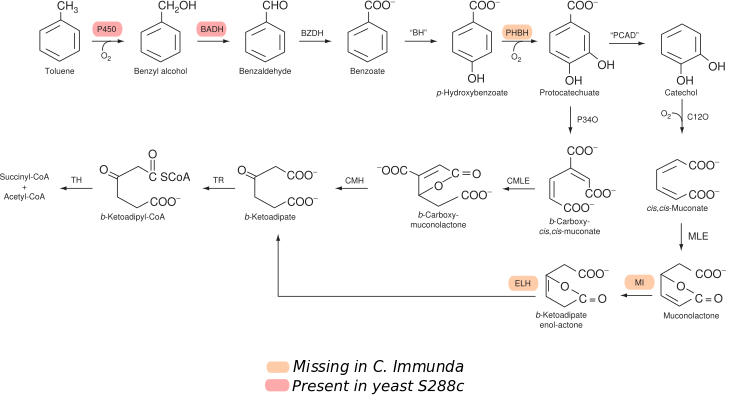
\includegraphics[width=360pt]{pics/toluenpathway.png}
	\caption[Toluene degradation pathway]
	{Toluene degradation pathway \cite{Parales2008}}
	\label{Toluendeg}
\end{figure}

Toluene (methylbenzene) is an aromatic hydrocarbon and natural product of diagenic origin and an important commercial chemical. The BTEX mixtures referred to in bioremediation applications contain benzene, ethylbenzene, toluene and xylenes. These toxic compounds are usually difficult to remove, due  to their wide dispersal in an ecosystem. 
%%%%%caros part of toluene
\\
A toluene degradation pathway in fungi is proposed for \textit{Cladophialophora saturnica} \cite{Badali2008} and in another previous study the connection between toluene metabolism and cytochrome P450 was established \cite{Luykx2003}. The examinations for the presence of genes belonging to the pathway for the toluene degradation (figure \ref{Toluendeg}) were done in comparison with the genome of the model yeast \textit{Saccharomyces cerevisiae} strain S288c. In the genome of \textit{S. cerevisiae}, only the first two enzymes of the pathway, cytochrome P450 and the benzyl alcohol dehydrogenase, are present. Three enzymes of the pathway are missing in  \textit{Cladophialophora immunda} \cite{Blasi2016, Parales2008}. \\


\section{Study of \textit{Cladophialophora immunda}}\label{study}
 \begin{figure}[H]
 	\centering	
 	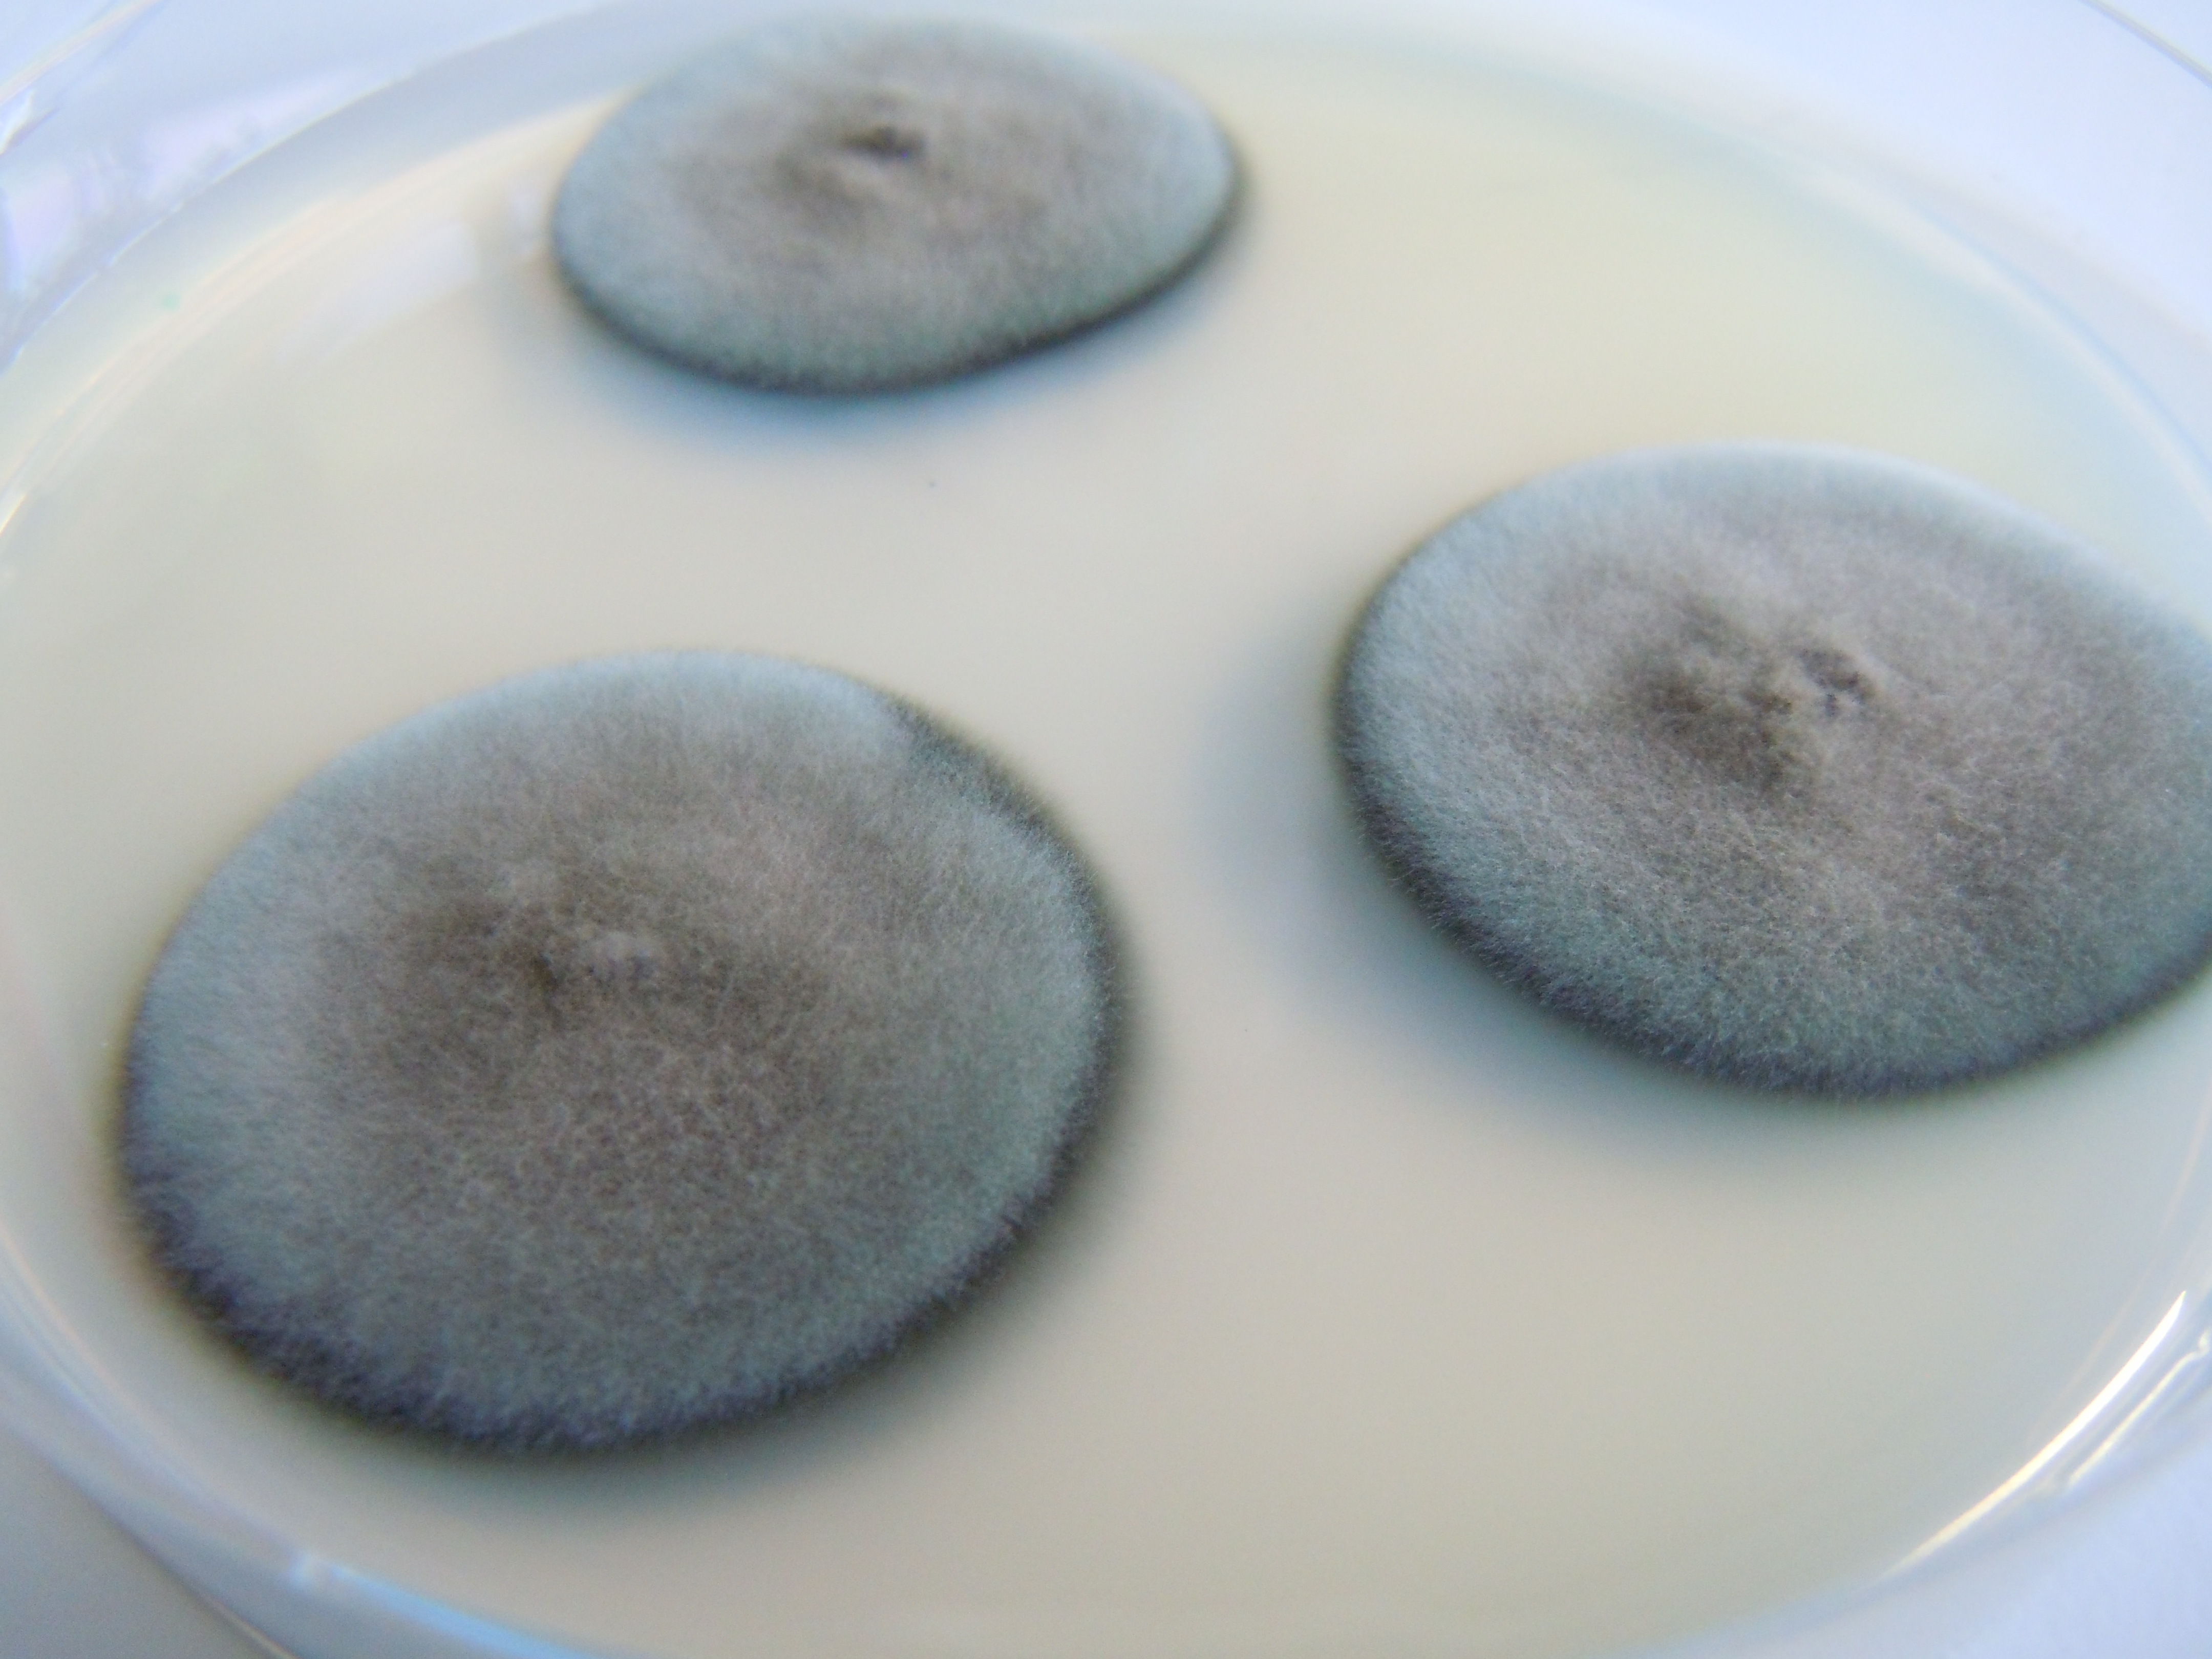
\includegraphics[width=300pt]{pics/cimmunda1.JPG}
 	\caption[\textit{Cladophialophora immunda}]
 	{\textit{Cladophialophora immunda}}
 \end{figure}
 
The black yeast \textit{Cladophialophora immunda} is known for the capability to grow on aromatic hydrocarbons and moreover for the ability to degrade hydrocarbons.\\
The genus \textit{Cladophialophora} belongs to the ascomycetes and forms two phylogenetic glades (\textit{Carrionii} and \textit{Bantiana}) in the family of \textit{Herpotrichiellaceae}, order \textit{Chaetothyriales}. \textit{Cladophialophora} is morphologically characterized by one-celled, ellipsoidal to fusiform, dry conidia arising through blastic, acropetal conidiogenesis and arranged in branched chains (figure \ref{fig:morph}). The genus includes species causing skin infections and other human diseases. \textit{C. immunda} is of special medical and biotechnological interest because it is frequently isolated both from humans and from contaminated soil \cite{Sterflinger2015, Badali2008}. 

\begin{figure}[H]
	\centering
	\begin{subfigure}{0.4\textwidth}
		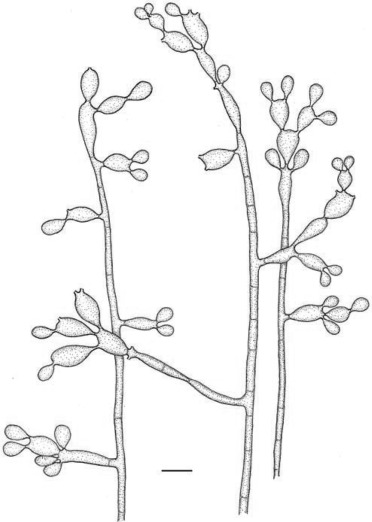
\includegraphics[width=130pt]{pics/cimmunda_morph} 
	\end{subfigure}
	\hspace*{0.01cm} 
	\begin{subfigure}{0.5\textwidth}
		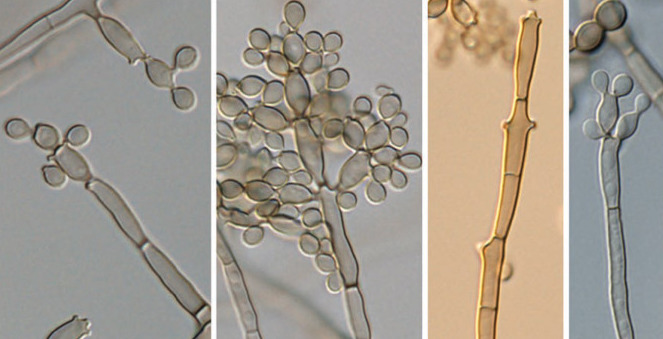
\includegraphics[width=230pt]{pics/cimmunda_morph2} 
	\end{subfigure}
	\hspace*{\fill} % separation between the subfigures
	\caption{Microscopic morphology of \textit{C. immunda} \cite{Badali2008}} \label{fig:morph}
\end{figure}

  
\textit{Cladophialophora immunda} was isolated from a gasoline
station, in a hydrocarbon rich environment, therefore the fungi is an
important candidate for bioremediation and for application in
biofilters \cite{Prenafeta-Boldu2001}.  \\ %barbaras work
To better understand the mechanisms of black yeasts and their effect of degrading
hydrocarbons, a preliminary study on bioremediation was undertaken. A collection of 163 strains of black yeast-like fungi from the CBS
Fungal Biodiversity Center (Utrecht, The Netherlands) was
screened for the ability to grow on hexadecane, toluene and
polychlorinated biphenyl 126 (PCB126) as the sole carbon and energy
source. These compounds were chosen as representatives of relevant
environmental pollutants.  The results indicated that the two strains
of \textit{C. immunda} and \textit{Exophiala mesophila} are able to
grow on media with toluene as a carbon source, confirmed by an increase
in CO$_2$ and a toluene decrease shown in figure \ref{GCresults}
\cite{BarbaraBlasi2015, Poyntner2014}.

\begin{figure}[H]
	\centering	
	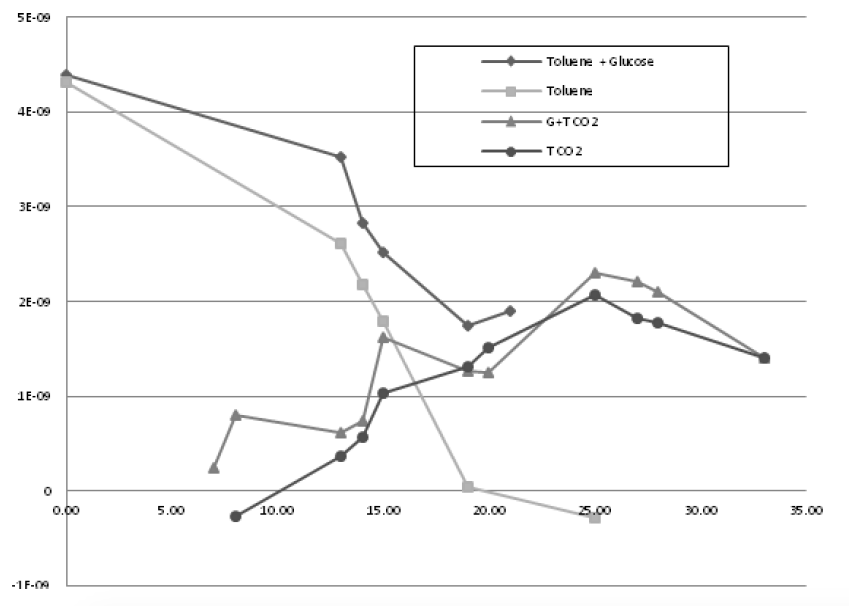
\includegraphics[width=400pt]{pics/GCresults.png}
	\caption[Toluene and CO$_2$ values for \textit{C. immunda}]
	{Toluene and CO$_2$ values for \textit{C. immunda}: Carbon equivalence [mol] of the two molecules was plotted against runtime [days] \cite{Poyntner2014}. }
	\label{GCresults}
\end{figure}

%%%% AIM OF THE THESIS %%%%%
This work uses the recently assembled genome of \textit{Cladophialophora immunda} and RNA-seq to annotate protein coding and non-coding genes. The protein sequence of the coding genes was used to elucidate their function. The RNA-seq data were obtained from \textit{Cladophialophora immunda} grown either on toluene or glucose as the sole carbon source. 
Accordingly the aim of this thesis is to examine the way in which the transcriptomes of \textit{Cladophialophora immunda} can be determined and to identify which genes are transcribed under different conditions. The major issue is to determine the pathways that allow \textit{C. immunda} to use toluene as carbon source.\\ 
The transcriptome data were obtained with RNA-seq performed by Ion Torrent technology coupled with the Ion Proton sequencer (Life Technologies, Carlsbad, CA) \cite{BarbaraBlasi2015}. 

\section{Transcriptome analysis}
The powerful technology RNA-sequencing and the analysis of transcriptomes, to know which gene is expressed, is an important method in this field. Transcriptome analysis enables the understanding of how sets of genes work together to form metabolic, regulatory and signalling pathways within a cell \cite{Xiong2006}.  
\subsection{RNA sequencing}
RNAs whole or fragmented are first converted into a library of cDNA fragments. Sequencing adaptors are added to each cDNA fragment at one or both ends. Each molecule is then sequenced in a high-throughput manner to obtain short sequences from one end (single-end sequencing) or both ends (pair-end sequencing). The reads are typically 30–400 bp, depending on the sequencing technology used. If the resulting sequence reads have been obtained, the first task of data analysis is to map the short reads from RNA-seq to the reference genome or to assemble them into contigs before aligning them to the genomic sequence to reveal transcription structure. The way of analysing transcriptomic data differs due to short reads also contain reads that span exon junctions or that contain poly(A) ends. Alignment can be also complicated for large transcriptomes as a result of matching multiple locations in the genome with a significant portion of sequence reads \cite{Wang2010}.  \\
An advantage of RNA-seq from earlier methods, such as microarrays, is the high throughput of current RNA-seq platforms, the sensitivity afforded by newer technologies and the ability to discover novel transcripts, gene models and non-coding RNA species \cite{Korpelainen2014}.  \\

\section{Bioinformatics methods}
The increasing use of next-generation sequencing methods leads to an overwhelming amount of data, which has to be stored, analysed and interpreted. Therefore bioinformatics methods are a necessary step in analysing transcriptomes. As RNA-seq is an active field of research producing new approaches and tools at a rapid pace, many alternative programs exist for each analysis step \cite{Korpelainen2014}. 

\subsection{Workflow System}
The data analysing steps were performed by different programs and tools, which may need specific data formats and external files. The multiple steps can be handled through scripting a reusable pipeline with defined inputs, outputs and parameters for each step. 

The software Snakemake was used to evolve the pipelines for genome annotation, functional annotation and enrichment analysis. Snakemake is based in Python language and can be used on a single core workstation as well as on a cluster without modifying the workflow. 
Snakemake's option "--dag" creates the directed acyclic graph (DAG) of executed jobs \cite{Koster2012}.   
\newline
Figure \ref{fig:DAG} gives an example of the DAG of the educed Snakemake file. Jobs (i.e. the execution of a rule) are depicted as nodes, a directed edge between two jobs means that the rule underlying the second job needs the output of the previous job executed before as an input file. A path represents a series of jobs that have to be executed sequentially.
\begin{figure}[H]
	\centering	
	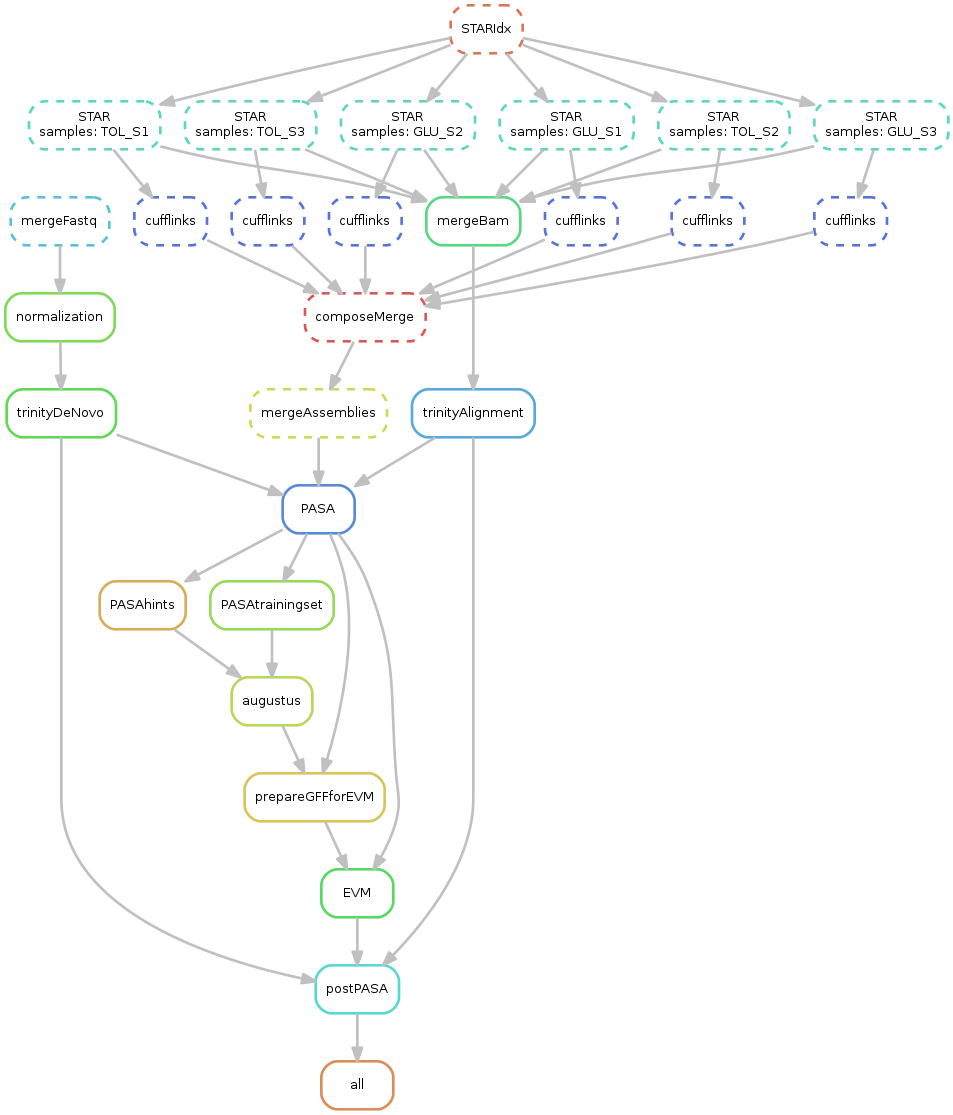
\includegraphics[width=430pt]{pics/DAG.png}
	\caption[Directed acyclic graph (DAG)]
	{Directed acyclic graph (DAG) of a Snakemakefile}
	\label{fig:DAG}
\end{figure}

\newpage
\setcounter{chapter}{2}\setcounter{section}{0}
\chapter*{Methods}
\addcontentsline{toc}{chapter}{Methods}
\section{Growth of \textit{Cladophialophora immunda}}
For the experimental conditions, the cultivation of \textit{Cladophialophora immunda} with glucose or toluene as carbon-source was chosen. \\
The \textit{Cladophialophora immunda} strain (CBS 110551) was isolated from a toluene-charged air biofilter inoculated with gasoline-polluted soil \cite{Prenafeta-Boldu2001}.  \\
\textit{Cladophialophora immunda} (CBS 110551) was cultured in malt extract agarose media (2 $\%$ malt extract, 2 $\%$ D-glucose, 0.1 $\%$ bacto-peptone and 2 $\%$ agar). \\
For the RNA-seq experiments, \textit{C. immunda} was grown in liquid culture in a modified Hartmans` mineral media with 2 $\%$ glucose or 1.35 mM toluene as carbon sources \cite{Hartmans1991}. The toluene was supplied through the air of a sealed flask in a 5 $\%$ solution in dibutylphtalate. The experiments duration was 90 days (growth with toluene) and one week (growth with glucose) at the temperature of 22 $^\circ$C at 100 rpm on an orbital shaker. Both experiments were performed in 3 biological replicates. At the end of the experiments the biomass was collected by centrifugation (5000 g per 15 minutes at 4 $^\circ$C), washed with RNAse free water, frozen in liquid nitrogen and stored at -80 $^\circ$C until use. \\

\begin{table}[h]
	\centering
	\begin{tabular}{c c | c c}
		\multicolumn{2}{c|}{Solution A} & \multicolumn{2}{c}{Solution B}  \\
		\multicolumn{2}{c|}{(1 litre demineralized water)}  & \multicolumn{2}{c}{(1 litre demineralized water)} \\
		\hline
		(NH$_4$)$_2$SO$_4$ & 200 g & K$_2$HPO$_4$ & 155 g\\
		MgCl$_2$.6H$_2$O & 10 g & NaH$_2$PO$_4$.2H$_2$O & 85 g \\
		EDTA & 1 g & &  \\
		ZnSO$_4$.7H$_2$O & 0.2g & & \\
		CaCl$_2$2H$_2$O & 0.1 g & & \\
		FeSO$_4$.7H$_2$O & 0.5 g & & \\
		Na$_2$MoO$_4$.2H$_2$O & 0.02 g & &\\                                
		CuSO$_4$.5H$_2$O & 0.02 g & & \\
		CoCl$_2$.6H$_2$O & 0.04 g & & \\
		MnCl$_2$.2H$_2$O & 0.1 g & & \\                          
	\end{tabular}
	\caption{Hartmans\textquotesingle mineral media}
\end{table}

The medium (1 litre of demineralized water) is compose by: \\
Solution A: 10 mL \\
Solution B: 25 mL \\
+ 0.02 $\%$ yeast extract as nitrogen source

\section{RNA-seq library preparation}
The work in the laboratory included the extraction of total RNA from 100 mg of fungal biomass with FastRNA PRO\textsuperscript{\texttrademark} RED KIT (MP Biomedicals) according to the instructions of the manufacturer. The mRNA was isolated with the Dynabeads\textsuperscript{\textregistered} mRNA DIRECT\textsuperscript{\texttrademark} Micro Kit (Ambion by Life Technologies) and the following transcriptome library preparation was performed with the Ion Total RNA-Seq Kit v2 (Life Technologies). 
Total RNA, isolated mRNA and the final cDNA library were all qualitatively and quantitatively evaluated by mean of Agilent 2100 Bioanalyzer (Agilent Technologies, Santa Clara, CA). The RNA-seq was performed by the Ion Proton\textsuperscript{\texttrademark} sequencer (Life Technologies) with the Ion PI Chip v2 (Life Technologies). 
The average read length of the six cDNA libraries was 175 bp for all five samples. Total reads generated per sample varied between 57,611,573 and 99,965,344. 

\section{Mapping Algorithm}\label{STAR}
The first step to understanding a genome structure is through genome mapping, which is a process of identifying relative locations of genes on a chromosome. When a read is mapped to reference genome, a sequence alignment is created \cite{Xiong2006}. The input files in this case were the preprocessed reads and in addition the reference sequence. \\
%%%%%Suffix tree
\subsection{Suffix Tree}
The rapid advance of new sequencing technology expand the scale and resolution of many biological applications like quantitative analysis of transcriptome where sequence reads must be compared to a reference. Various algorithms to optimally solve the mapping problem were developed in the last few years. Some of them are based on hash tables and the others are based on suffix trees. Both approaches first identify exact matches and subsequently build inexact alignments supported by exact matches. Finding exact matches rely on a representation of suffix tree. 
The advantage of suffix trees over hash tables is that by using a tree the alignment to multiple identical copies of substring in the reference has to be done only once. Because the identical copies collapse on a single path in the tree, otherwise in a hash table index an alignment must be performed for each copy \cite{Li2010}. \\
A suffix tree is a data structure that stores all the suffixes of a string to enabling fast string matching. The time complexity of determining if a query has an exact match against a tree is linear in the length of the query, independent of the length of the reference sequence. Nonetheless a tree takes \textit{O(L$^2$)} space, where \textit{L} is the length of reference. To reduce the space a approach to achieves linear space while allowing linear time searching is used. In theory it is possible to represent a suffix tree \textit{L log$_2$L + O (L)} bits using rank-selection operations. To solve this space efficient implementation,  an enhanced suffix array was derived that consists of a suffix array and several auxiliary arrays. A suffix array can be regarded as an implicit representation of suffix tree and has an identical time complexity to suffix tree in finding exact matches \cite{Li2010}. 

%%%%%Star specific approach
\subsection{\textit{STAR} specific approach}
Mapping is computationally intensive, that is why the program \textit{STAR} was chosen. \textit{STAR} (Spliced Transcripts Alignment to a Reference) is a spliced alignment program which runs very fast. The benefits of \textit{STAR} are largely based on the Maximum Mappable Length approach. \\
The algorithm Maximum Mappable Length (\textit{MML}) was developed to align reads to the genome. The idea of \textit{MML} approach is to search a Maximum Mappable Prefix (\textit{MMP}). Given a read sequence \textit{R}, read location \textit{i} and a reference genome sequence \textit{G}, the \textit{MMP(R,i,G)} is defined as the longest substring  
\[
[R_{i} , R_{i+1} , ... , R_{i+MML-I} ]
\]
which matches exactly one or more substrings of G, where \textit{MML} is the maximum mappable length. 
Starting from the first base of the read the algorithm finds the \textit{MMP}. If \textit{MMP} can not be mapped contiguously to the genome because of an splice junction, this first seed will be mapped to a donor splice site. The \textit{MMP} search is repeated for the unmapped portion of the read, which will be mapped to an acceptor splice site.
The difference to other algorithm is to align the non-contiguous sequences directly to the reference genome, which accelerated the process to map \cite{Dobin2013}. \\
\textit{STAR} splits a read and find the best portion that can be mapped for each piece. Then it maps the remaining portion, which can be far away in the case of a splice junction. The maximum mappable seed search looks for exact matches and uses the genome in the form of uncompressed suffix arrays. The second step of \textit{STAR} stitches the seeds together within a given genomic window and allows mismatches, indels and splice junctions. The seeds from read pairs are handled concurrently at this step in order to increase sensitivity \cite{Dobin2013, Korpelainen2014}. 

\section{Count Algorithm}\label{featurecount}
 %%FEATURE COUNTS
Read mapping results have to be summarized in terms of read coverage for genomic features of interest. Read counts are required for statistical methods like differential expression analysis.The approach of counting the number of mapped reads to annotation was accomplished by the program \textit{featureCounts}. \\
\textit{featureCounts} performs precise read assignment by comparing mapping location of every base in the read or fragment with the genomic region spanned by each feature. It takes account of any gaps like insertions, deletions, exon–exon junctions or fusions) that are found in the read. 
The input for \textit{featureCounts} consists of aligned reads in Sequence Alignment/Map (sam) or Binary Alignment/Map (bam) format and a list of genomic features in general feature format (gff). The read alignment and the feature annotation should correspond to the same reference genome, which is a set of reference sequences representing chromosomes or contigs. \textit{featureCounts} supports strand-specific read counting with the option "-s". 
\begin{figure}[ht]
	\centering	
	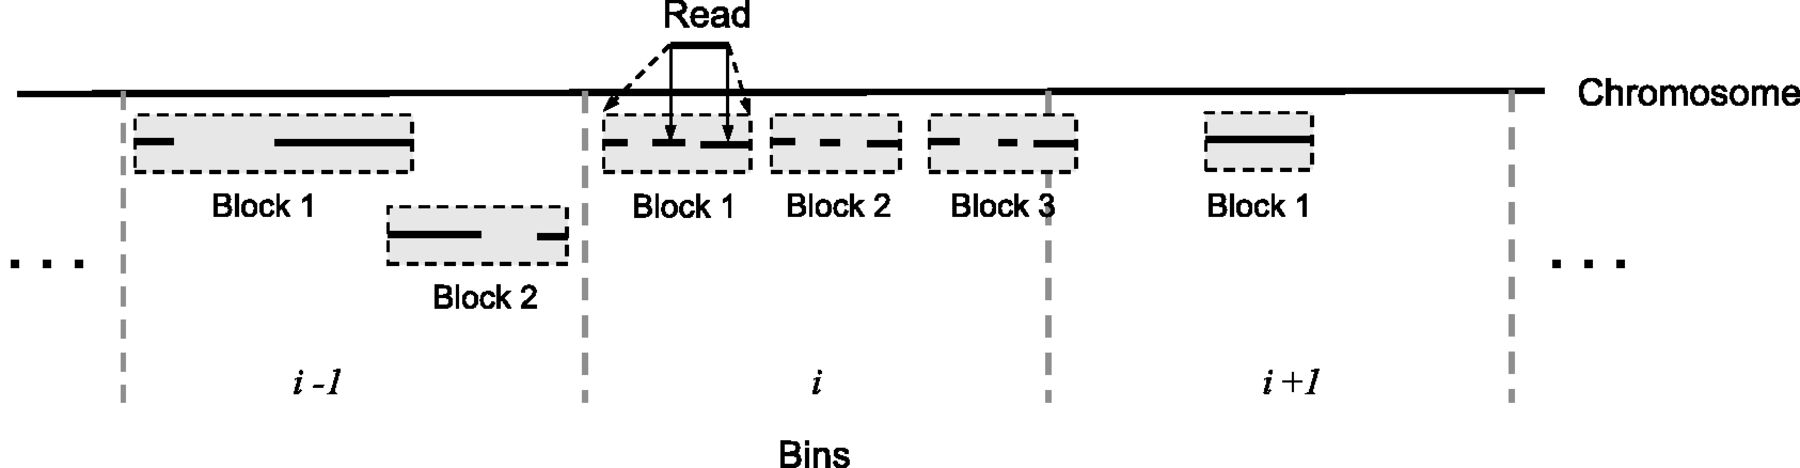
\includegraphics[width=400pt]{pics/featurecounts}
	\caption[Approach of software \textit{featureCounts}]
	{Approach of \textit{featureCounts}: genome bins and feature blocks \cite{Liao2014}. }
	\label{fig:featurecounts}
\end{figure}

The algorithm is starting to generate a hash table for the reference sequence names. This enables that the reference sequence names are found to match in the input of sam/bam-files and gff-annotation quickly. Next the features in each reference sequence are sorted by their start position and a two-level hierarchy is created. Each chromosome is divided into non-overlapping 128kb bins. Features are assigned to bins according to their start positions and grouped into blocks within each bin. The query read is compared first with genomics bins, then with feature blocks within any overlapping bins and then with features in any overlapping blocks. This approach is shown in the illustration \ref{fig:featurecounts} \cite{Liao2014}. 

\section{Differential Expression Algorithm}
%%LIMMA
Differential expression analysis refers to identification of genes or type of genomic features such as transcripts or exons, that are expressed in significantly different quantities in distinct groups of samples. In this study two sets of biological conditions, growth on toluene vs. growth on glucose, were compared with R/BioConductor packages \textit{limma}.\\

\begin{figure}[H]
	\centering	
	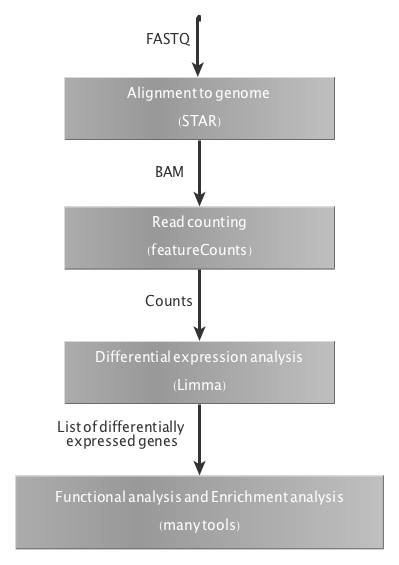
\includegraphics[width=150pt]{pics/diffgraph}
	\caption[Steps of differential expression analysis]
	{Steps of differential expression analysis}
\end{figure}

The first step of differential analysis is achieved by mapping RNA-seq data with \textit{STAR} (\ref{STAR}). The data input to \textit{limma} should be raw counts produced by \textit{featureCounts} (\ref{featurecount}). %\HT{FEATURECOUNT RETURNS RAW COUNTS AND NOT RPKM}
\textit{Limma} was then used to find differentially expressed genes. \\
The software is based on the concept of linear models with the idea to model the expression of each gene as a linear combination of some different explanatory factors. For the experiment on \textit{C. immunda} the linear model for each gene assembled by the measured gene expression (\textit{y}) is equal to the intercept (\textit{a}) representing the average expression level of the gene when the factor (\textit{condition}) is in its reference state plus the error term (\textit{e}): 
\[y = a + b * condition + e\]
A generalized linear model (GLM) is a more flexible version of a standard linear model that allows the distribution of the response variable to be different from the normal distribution used in standard linear regression. GLM assume that the read counts are distributed according to the negative binomial distribution. 
Accordingly the linear model should be written in matrix form, where the expression level (\textit{y}) is equal to experimental factor (\textit{X}) multiplied by the vector of parameters to be estimated from the data ($\beta$) plus the error term ($\varepsilon$):
\[ \mathrm{ y = X * \beta + \varepsilon}\]
Hence a contrast matrix has to be set up that describes which comparisons wants to be done. The advantages of \textit{limma} is that it can account for more than one varying experimental factor using a generalized linear modelling framework, it is very fast and memory-intensive \cite{Ritchie2015}. 


\section{Enrichment Approach}
%\HT{UNCLEAR: Trough Enrichment Analysis a list of over-represented molecular functions, biological processes and cell locations, that can then be used to test whether genes are regulating biochemical or cellular pathway, is provided. Enrichment analysis is a necessary step after data analysis for more detailed annotations about differentially expressed genes, so that a biological meaning can be postulated. \\} 
Enrichment Analysis is a method to identify a group of genes or proteins of over-represented molecular functions, biological processes and cell locations. After differential expression analysis genes are linked to biological pathways and the additive changes of expression within gene sets are shown.\\
\ \\
Functional annotation elements are identified with R-packages Gene Set Enrichment Analysis (GSEA) \cite{Subramanian2005} and Gene Ontology (GO) and the metabolic pathways by Kyoto Encyclopedia of Genes and Genomes (KEGG). 
A custom script was used to summarize the list of significantly overrepresented GO terms and data are graphically represented with R. \\
\ \\
Gene Ontology classifies genes according to the biological process, cellular component and molecular function. It defines terms with gene products call GO terms, which are more or less detailed, depending on the state of knowledge or annotation. 
Each GO term has a term name, a unique identifier, the ontology it belongs to, synonyms including exact related ones and alternative unique identifiers, a definition including the source, a comment, the subset the terms belong to and community comments. The ontology is structured as a directed acyclic graph and each term has defined relationships to one or more other terms in the same domain. To kept in mind that the problem with using the GO terms is that a certain gene can map to several GO terms \cite{Ashburner2000}. \\
\ \\
Kyoto Encyclopedia of Genes and Genomes is a collection of databases dealing with biological pathways, genomes, diseases, drugs, and chemical substances. KEGG links genomic information with higher order functional information by computerizing current knowledge on cellular processes and by standardizing gene annotations. KEGG consists of three databases where the informations are stored. The genes database includes the genomic information, which is a collection of gene catalogs for all the completely sequenced genomes and some partial genomes with up-to-date annotation of gene functions. The higher order functional information is saved in the pathway database, which contains graphical representations of cellular processes, such as metabolism, membrane transport, signal transduction and cell cycle. The third one is the ligand database for the information about chemical compounds, enzyme molecules and enzymatic reactions \cite{kanehisa2000}. 

\section{Pipeline implementation}
%overview of the pipeline used where all paramaters and thresholds are use. this leads us than to the results. 
The six data sets used was downloaded from the sequencer-server, three data sets %\HT{bezieht sich auf?} 
were the transcriptomes of \textit{Cladophialophora immunda} cultivated with glucose as carbon-source and the other three data sets with toluene. \\
Before implementing the workflow system a comparison of publications, different programs and tools were done. The choice of a suitable program depended on the kind of analysis and the performance and the amount of time it required. Another important issue was the option available of the used program. \\
In the beginning the reads' origin was identified by aligning them to the reference genome with \textit{STAR}. Mapped reads were used to perform transcript assembly with the softwares \textit{Cufflinks} and\textit{Trinity Genome Guided}. \textit{Trinity} also was employed for mapping-free transcript assembly. With the produced assemblies from \textit{Cufflinks} and\textit{Trinity}, the Program to Assembly Spliced Alignments (\textit{PASA}) performed the spliced alignment mapping. \textit{PASA} assemblies were utilized to create hints for the location of introns and exons. Those hints were integrated in a hint-based run of \textit{Augustus}. Evidence Modeler (\textit{EVM}) was used to combine weighted predictions. The last step was a annotation update implemented by \textit{PASA}, where the output of \textit{EVM} compared to \textit{PASA} alignment assemblies and generated a updated gene set \cite{Haas2011, Steijger2013, Linde2015}.  \\
Figure \ref{fig:pipeline} shows the draft of the entire workflow system for genome annotation with transcriptomic data. The inputs are the transcriptomes from RNA-Seq in bam-format, the genome in fasta-format and the \textit{deNovo} annotation data in gff3-format. After runs of the different steps the output is an annotation file in gff3-format.

\begin{figure}[H]
	\centering	
	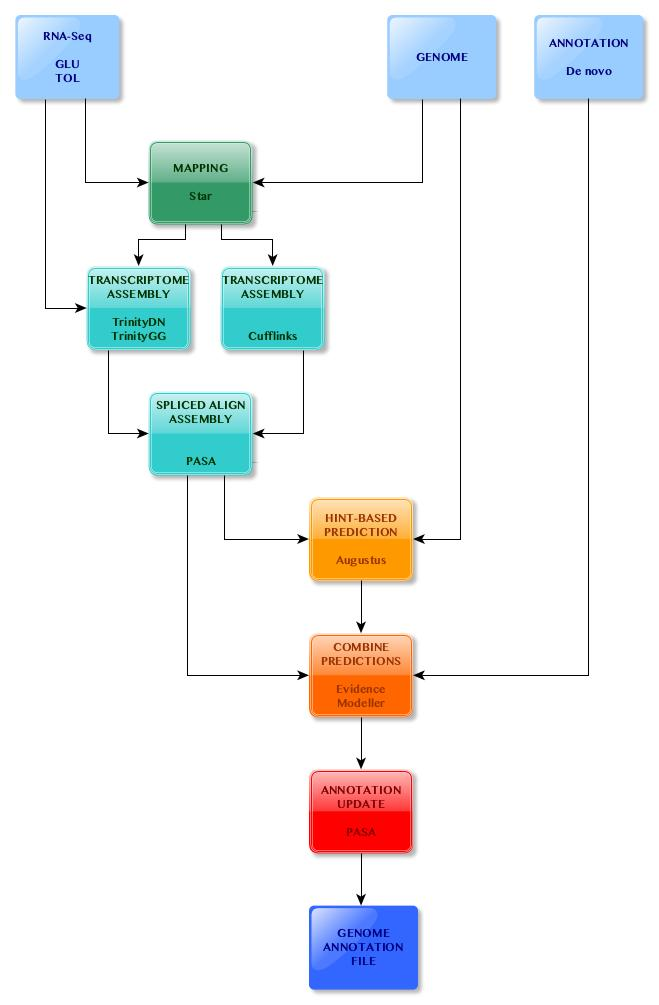
\includegraphics[width=310pt]{pics/pipeline}
	\caption[Genome Annotation Workflow]
	{Genome annotation workflow system}
	\label{fig:pipeline}
\end{figure}

%%%% Overview
\subsection*{Mapping}
\subsubsection*{\textit{STAR}}
The execution of \textit{STAR} allocated in two parts, building a reference index and mapping. Before running \textit{STAR} mapping it was obtained a reference index of the genome. Mapping of the reads was executed without the soft clip aligning at reference ends. The mapped reads needed to be sorted by \textit{Samtools}.

\subsection*{Transcriptome Assembly}
The goal of RNA-seq assembly is to reconstruct full-length transcripts based on sequenced reads. Transcript assembly answers the questions about exon regions and splice site. Several transcripts may overlap at different regions or there may be multiple copies of the same transcript. \\
There are two ways of performing transcriptome assembly. If there is a reference genome, it can be realised to guide the assembly, where the assembly task consists of solving which mapped reads correspond to which transcript. The second possibility is to perform \textit{deNovo} assembly \cite{Korpelainen2014}.  

\subsubsection*{\textit{Cufflinks}}
The software packages \textit{Cufflinks} can be used for \textit{ab intio} reconstruction. The program within in this packages \textit{Cufflinks} assembles transcriptomes from RNA-Seq data. \textit{Cufflinks} reports the smallest possible set of isoforms. The program \textit{Cuffmerge} was used to merge the multiple assembled transcriptomes into a master transcriptome \cite{Trapnell2010}. \\
The rule \textit{Cufflinks} was implemented with the following option and values: the maximum intron length (2000) and the minimum intron length (30), the maximum number of fragment a locus may have before skipped (10000) and the library-type ff-firststrand.

\subsubsection*{\textit{Trinity}}
\textit{Trinity} consists of three separate programs: \textit{Inchworm}, which construct initial contigs, \textit{Chrysalis} which clusters the contigs produced by \textit{Inchworm} and creates a de Bruijn Graph for each locus and \textit{Butterfly}, which extracts the isoforms within each de Bruijn Graph. 
Each node of a de Bruijn Graph is associated with a (k -1)-mer. Two nodes A and B are connected if there is a k-mer whose prefix is the (k -1)-mer of the node A and the suffix is (k - 1)-mer of the node B. The k-mers create edges in the Buijn graph \cite{Korpelainen2014}. The k-mers is fixed to be 25 in \textit{Trinity} the version 2.0.2.
\textit{Jellyfish} is the software, which calculates the k-mers and therefore maximum memory has to be defined \cite{Grabherr2011}. 
%%%%% Manfred grabherr
\ \\
\textit{Trinity} was executed genome-guided and \textit{deNovo}. For genome-guided \textit{Trinity} the mapped reads in bam-format and for the \textit{deNovo} approach the raw reads in fastq-format were used. In both the option for strand-specific RNA-Seq read orientation for single end forward was required. 

\subsubsection*{\textit{PASA}}
Program to Assembly Spliced Alignments (\textit{PASA}) annotates protein-coding genes and alternatively splicing isoforms automatically. The goal of \textit{PASA} is to find for each alignment the largest assembly, which is used to create gene models or to modify existing gene models \cite{Haas2003}. 
Further reconstructed assemblies are the input into \textit{PASA} tool. Then \textit{PASA} aligns these newly assembled transcripts to the genome using the software \textit{GMAP}. Next \textit{PASA} filters invalid alignments and those transcripts more likely resulting as artifacts of the RNA-seq assembly process and reconstructs more complete transcripts using its alignment assembly algorithm \cite{Haas2011}. \\
The reconstructed inputs for the \textit{PASA} run were \textit{Trinity deNovo} assemblies, \textit{Trinity genome-guided} assemblies and \textit{Cufflinks} transcript structures. 

\subsection*{Gene Prediction}
\subsubsection{\textit{Augustus}}
\textit{Augustus} is an \textit{ab intio} gene predictor, where only a genomic sequence is needed as input information. In addition it is possible to use hints of various information. For the prediction \textit{Augustus} combines genomic sequence alignments and alignments of expressed sequenced tags (EST).\\
Expressed Sequence Tag (EST) was evolved in early days of genome assembly. First the same assemblers where used for transcriptomes, but there a fundamental differences between genome assembly and transcriptome assembly. In the genome assembly the ideal output is a linear sequence representing each genomic region, whereas in the transcriptome assembly the gene is most naturally described as a graph \cite{Korpelainen2014}.  \\
 The model underlying the program is generalized hidden Markov model (GHMM). HMMs and GHMMs for gene prediction define a probability for each pair ($\mathrm{\varphi}$,s) of a sequence (s) and a gene structure ($\mathrm{\varphi}$). Before starting the program \textit{Augustus} it is necessary to train the model \cite{Stanke2006}.  \\
The trainingset was created from \textit{PASA} assemblies by executed the program "pasa\_asmbls\_to\_training\_set.dbi" included in \textit{PASA} package. For the additional file of hints the location of introns were filtered from \textit{PASA} assemblies. Subsequently \textit{Augustus} was started and after more than 24 hours, the output was a complete gene prediction in ggf-format. 

\subsubsection{\textit{Evidence Modeler}}
The Evidence Modeler (\textit{EVM}) is an automated eukaryotic gene structure annotation tool. \textit{EVM} reports eukaryotic gene structures by using weighted evidence combining technique. The evidence utilized by \textit{EVM} corresponds to \textit{ab initio} gene predictions and transcript alignment \cite{Haas2008}.  \\
The assembly of \textit{PASA} (weight = 10), the \textit{Augustus} prediction (weight = 5) and the \textit{deNovo} Annotation (weight = 1) were combined by \textit{EVM}.

\subsubsection{\textit{Pasa Annotaion Update}}
Again Program to Assembly Spliced Alignments (\textit{PASA}) was used to update the \textit{EVM} consensus prediction by adding UTR annotations and models for alternatively spliced isoforms.


%%%%%%% RESULTS %%%%%%
\newpage
\setcounter{chapter}{3}\setcounter{section}{0}
\chapter*{Results}
\addcontentsline{toc}{chapter}{Results}
%Presentation of raw results
The average mean read length was 140 bp and the total reads generated per sample varied between 85,080,007 and 94,144,127. 
\begin{table}[H]
	\centering
	\begin{tabular}{|c|c|c|}
		\hline
		\textbf{Samples} & \textbf{Total Reads} & \textbf{Mean Read Length [bp]}  \\
		\hline
		GLU1 & 85.1M & 133 \\
		\hline
		GLU2 & 94.1M & 147  \\
		\hline
		GLU3 & 85.8M & 140  \\
		\hline
		TOL1 & 87.8M & 159  \\
		\hline
		TOL2 & 78.0M & 134  \\
		\hline
		TOL3 & 84.6M & 130  \\
		\hline
	\end{tabular}
	\caption{RNA Sequencing Read Summary}
\end{table}

\section{Genome Annotation}
%%%Annotation ergänzen
Annotations connect novel RNA sequencing data with biological information about the same transcripts derived from other studies. If a reference genome is available, genomic coordinates are normally associated with various form of annotation information through databases. Otherwise the mapping coordinates are given from an alignment. 
\begin{table}[H]
	\centering
\begin{tabular}{c c c|c}
	\textbf{\textit{C. immunda}} & & \textbf{Genes} & \textbf{Proteins} \\
	\textbf{CBS83496}& & 14,438 & 16,812   \\ 
	
	
\end{tabular}
\caption{Genome Annotation}
\end{table}

\section{Up- and Down-regulated genes}
Differential expression analysis was used to prepare lists of up- and down-regulated genes. In order to filter significant results of differential expressed genes, a threshold for the \textit{p}-value and \textit{logFC}-value (\textit{logFoldChange}) was set. \\
The \textit{p}-value is defined as the probability of the obtaining results and is used in hypothesis testing. The threshold value for \textit{p} is called the significance level. The \textit{FoldChange}-value is used to determine two data sets reflecting gene expression measured under different conditions. It´s logarithm is called \textit{logFoldChange}, which is more attractive for differential expression because positive values indicate up- and negative values indicate down-regulation. 
\[
\textit{Expression level B = Expression level A * foldChange}
\]
\[
\textit{logfoldChange = log2(foldChange)}
\]
%~\HT{sicherstellen dass du p-value, foldchange and log foldchange nicht verwerchselt}
If the result is 0.2, it means that the expression level in the experimental condition (TOL-samples) is 0.2-fold the expression as in the control condition (GLU-samples). \\
For the up-regulated data set threshold was set by a p-value less than 0.2 and the logFC-value (logFoldChange) greater than zero. For the down-regulated dataset threshold was set again by a p-value less than 0.2 but an logFC-value less than zero. \\

%%%%Overview most up-and down regulated genes
\underline{\textbf{10 most significantly Up- and Down-regulated genes}} 
\begin{table}[H]
	\centering
	\scriptsize
	\begin{tabular}{c|c|c|c|c|c|c}
		\textbf{geneID}& \textbf{logFC}&\textbf{AveExpr}&\textbf{t}&\textbf{P.Value}&\textbf{adj.P.Val}& \textbf{B}\\
		\hline
JSEJ01000027.1.121	&9,157671427&	11,01902243&	34,19677788&	4,59E-17&	3,92E-13&	28,15287351\\
JSEJ01000048.1.3&	8,135554813	&11,15870924&	30,84561682&	2,56E-16&	1,09E-12&	26,80565492\\
JSEJ01000128.1.27&	8,264361041&	8,24645472&	26,0280989&	4,29E-15&	1,22E-11&	24,15678934\\
JSEJ01000047.1.83&	6,143951797&	9,487939172&	24,95531824&	8,60E-15&	1,54E-11&	23,82051174\\
JSEJ01000040.1.6&	8,353205867&	6,693442984&	24,88192941&	9,03E-15&	1,54E-11&	23,18910965\\
JSEJ01000118.1.44&	6,055216556&	10,15304114&	23,86371332&	1,80E-14&	2,56E-11&	23,16026207\\
JSEJ01000012.1.35&	5,977114267&	12,65195266&	23,00250399&	3,29E-14&	3,29E-11&	22,58014797\\
JSEJ01000031.1.43&	6,754060011&	11,71227935&	22,92972613&	3,47E-14&	3,29E-11&	22,54452776\\
JSEJ01000113.1.50&	8,03548922&	10,60107357&	22,57155602&	4,49E-14&	3,83E-11&	22,30063571\\
JSEJ01000070.1.66&	8,508993803&	6,164674619&	22,2024474&	5,89E-14&	4,24E-11&	21,53678647\\
		\hline
		\end{tabular}
	\caption{10 most significantly Up-regulated genes}
\end{table}

\begin{table}[H]
	\centering
	\scriptsize
	\begin{tabular}{c|c|c|c|c|c|c}
		\textbf{geneID}& \textbf{logFC}&\textbf{AveExpr}&\textbf{t}&\textbf{P.Value}&\textbf{adj.P.Val}& \textbf{B}\\
		\hline
		JSEJ01000100.1.24&	-7,498665272&	7,747744106&	-22,98902806&	3,32E-14&	3,29E-11&	22,30611909\\
		JSEJ01000161.1.20&	-8,866531212&	6,185450242	&-21,75485658	&8,22E-14&	4,24E-11&	21,14599408\\
		JSEJ01000037.1.86&	-5,635055473&	8,551635429	&-21,08356096&	1,37E-13&	5,58E-11&	21,25535901\\
		JSEJ01000146.1.21	&-5,064637844&	9,170287113	&-19,05864813&	7,10E-13&	1,73E-10&	19,74278703\\
		JSEJ01000071.1.25	&-6,174423645&	7,057845126	&-18,85738485&	8,44E-13&	1,95E-10&	19,43283451\\
		JSEJ01000079.1.8	&-5,546577865&	9,934645785	&-18,34271713&	1,32E-12&	2,50E-10&	19,14942065\\
		JSEJ01000003.1.28&	-5,718439007&	7,347779099	&-17,74081308&	2,26E-12&	3,47E-10&	18,55773184\\
		JSEJ01000022.1.51&	-7,925562894&	6,932767343	&-17,42614263&	3,02E-12&	4,16E-10&	18,15011866\\
		JSEJ01000125.1.1&	-5,054168871&	6,687468173	&-17,19210644&	3,75E-12&	4,78E-10&	18,06479201\\
		JSEJ01000039.1.91&	-4,286585186&	10,59182994	&-16,99691044&	4,50E-12&	5,47E-10&	17,97012785\\
		\hline
	\end{tabular}
	\caption{10 most significantly Down-regulated genes}
\end{table}

Overall, the first 500 differentially expressed genes were considered. \\
To visualize the correlation of the samples and check for potential outliers a correlation heatmap and principal component (PCA) plot was created. \\
Heatmap using a color scale to displays the expression values of the genes. Genes are arranged in columns (samples) and rows (features) as in the data matrix. Each feature-sample pair is represented with a small rectangle that is coloured according to its expression. \\
The results of the correlation between the different samples are presented in the heatmap in figure \ref{fig:heatmap}. The dendrograms along the sides show how the samples and the features are independently clustered. Light colour like yellow indicates a good relation between the samples. The darker the colour, the lower is the correlation. \\
%~ \HT{bitte klarer darstellen:} 
Principal component analysis is based on finding which samples have the strongest correlation. It is a linear transformation method to show the variance in the data set. As figure \ref{fig:pca} shows a variance of 94$\%$ between the glucose and toluene samples. On y-axis the variance between the samples is 2$\%$. 
\ \\

%\begin{figure}[H]
%	\centering	
%	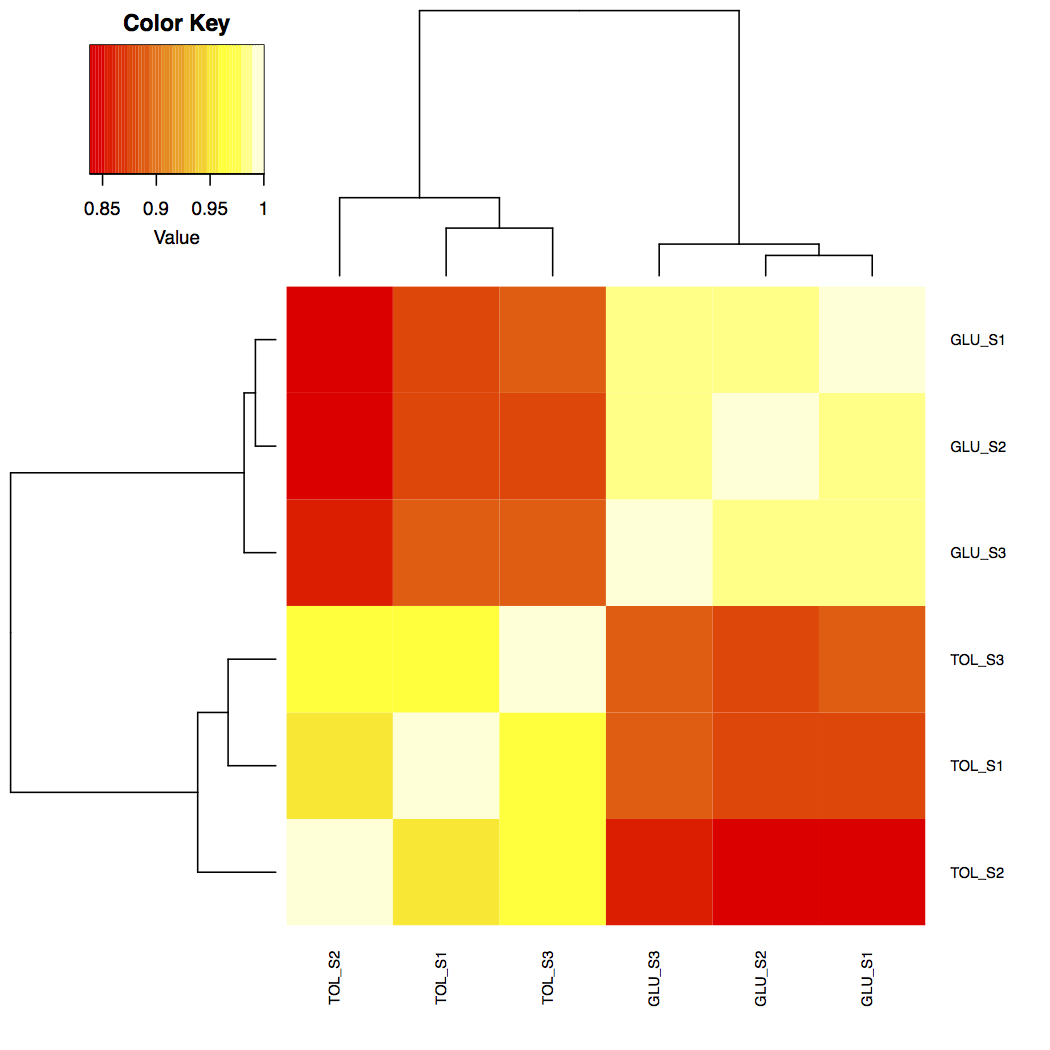
\includegraphics[width=250pt]{pics/heatmap2}
%	\caption[Correlation heatmap of the samples]
%	{Correlation heatmap of the samples}
%	\label{fig:heatmap}
%\end{figure}
%
%
%\begin{figure}[H]
%	\centering	
%	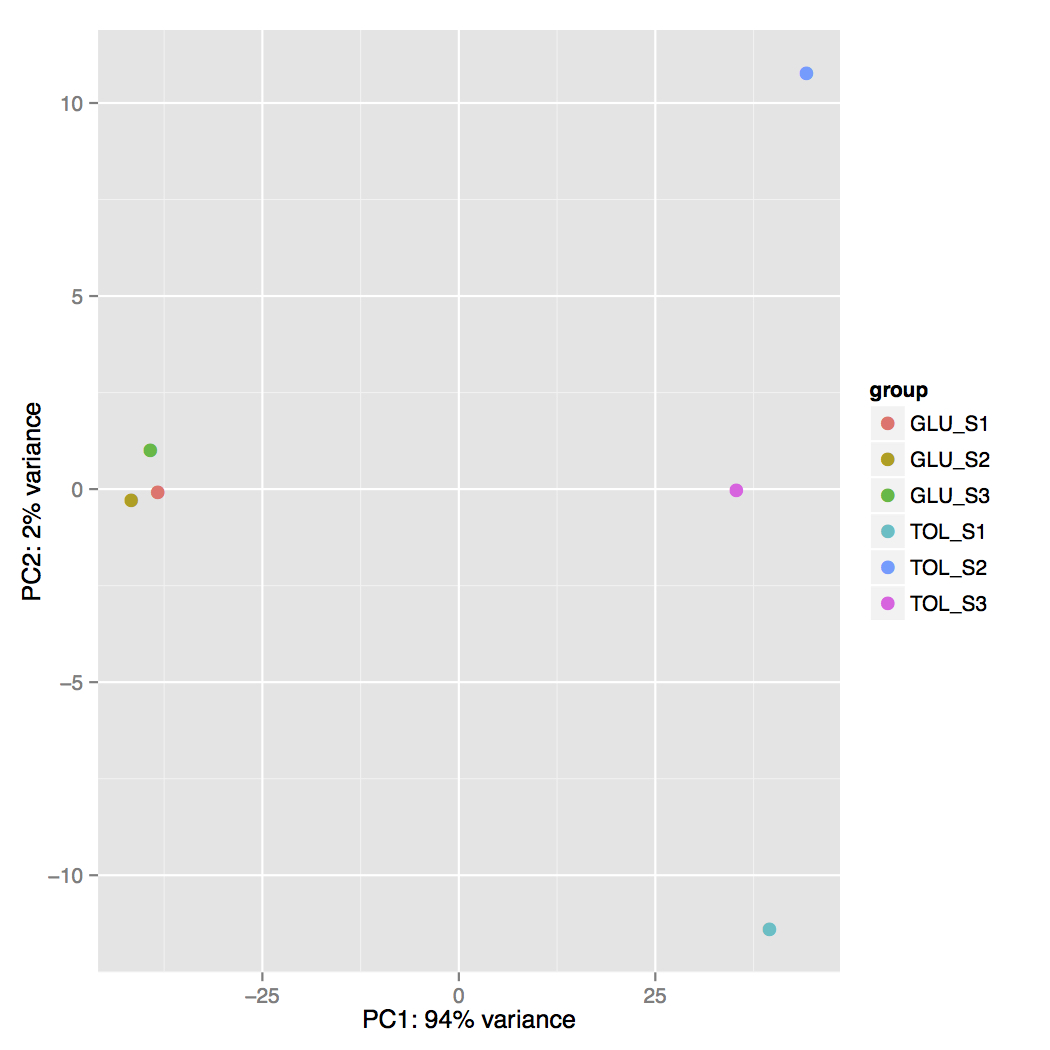
\includegraphics[width=250pt]{pics/PCA}
%	\caption[PCA]
%	{PCA}
%	\label{fig:pca}
%\end{figure}

\begin{figure}[H]
	\centering
	\begin{subfigure}{0.4\textwidth}
		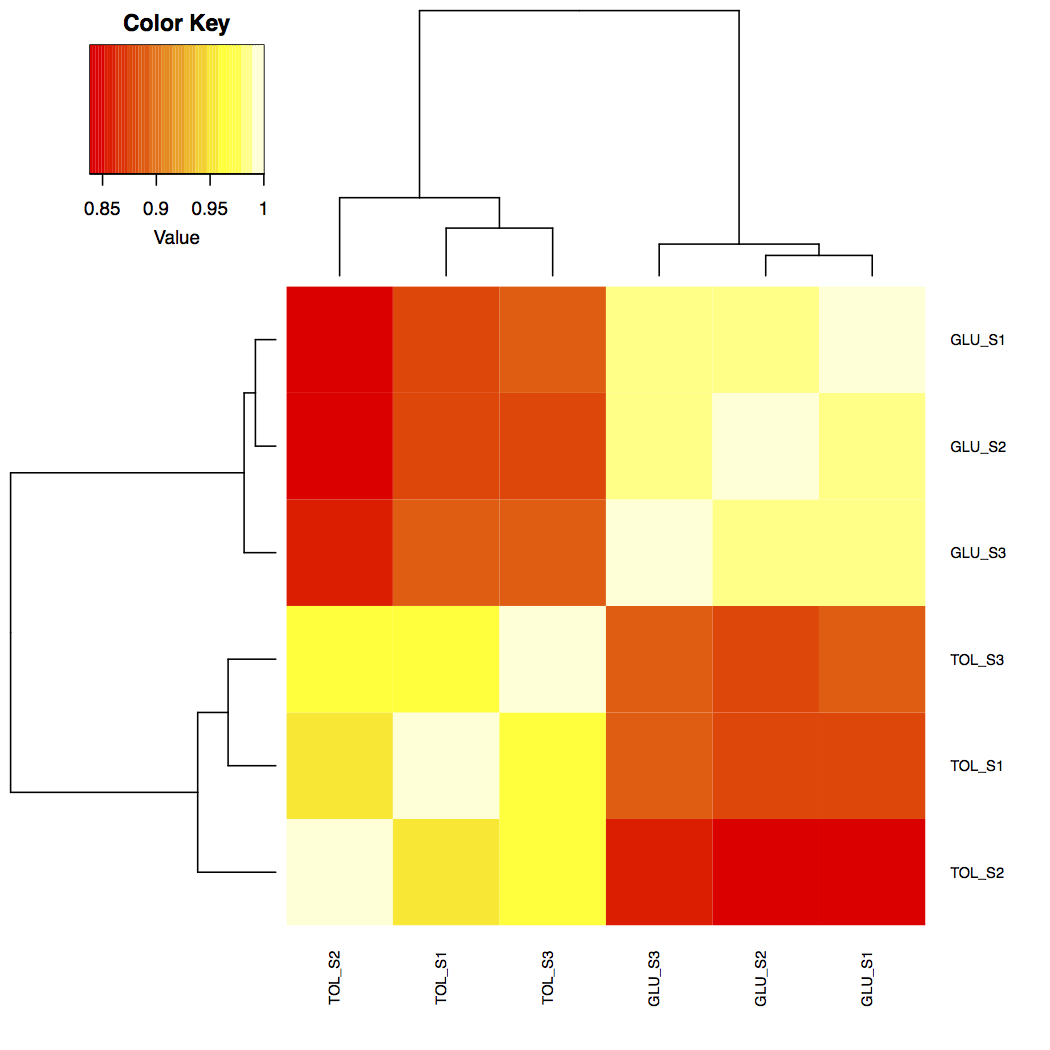
\includegraphics[width=200pt]{pics/heatmap2}
		\caption{Correlation heatmap} \label{fig:heatmap}
	\end{subfigure}
	\hspace*{1cm} 
	\begin{subfigure}{0.5\textwidth}
		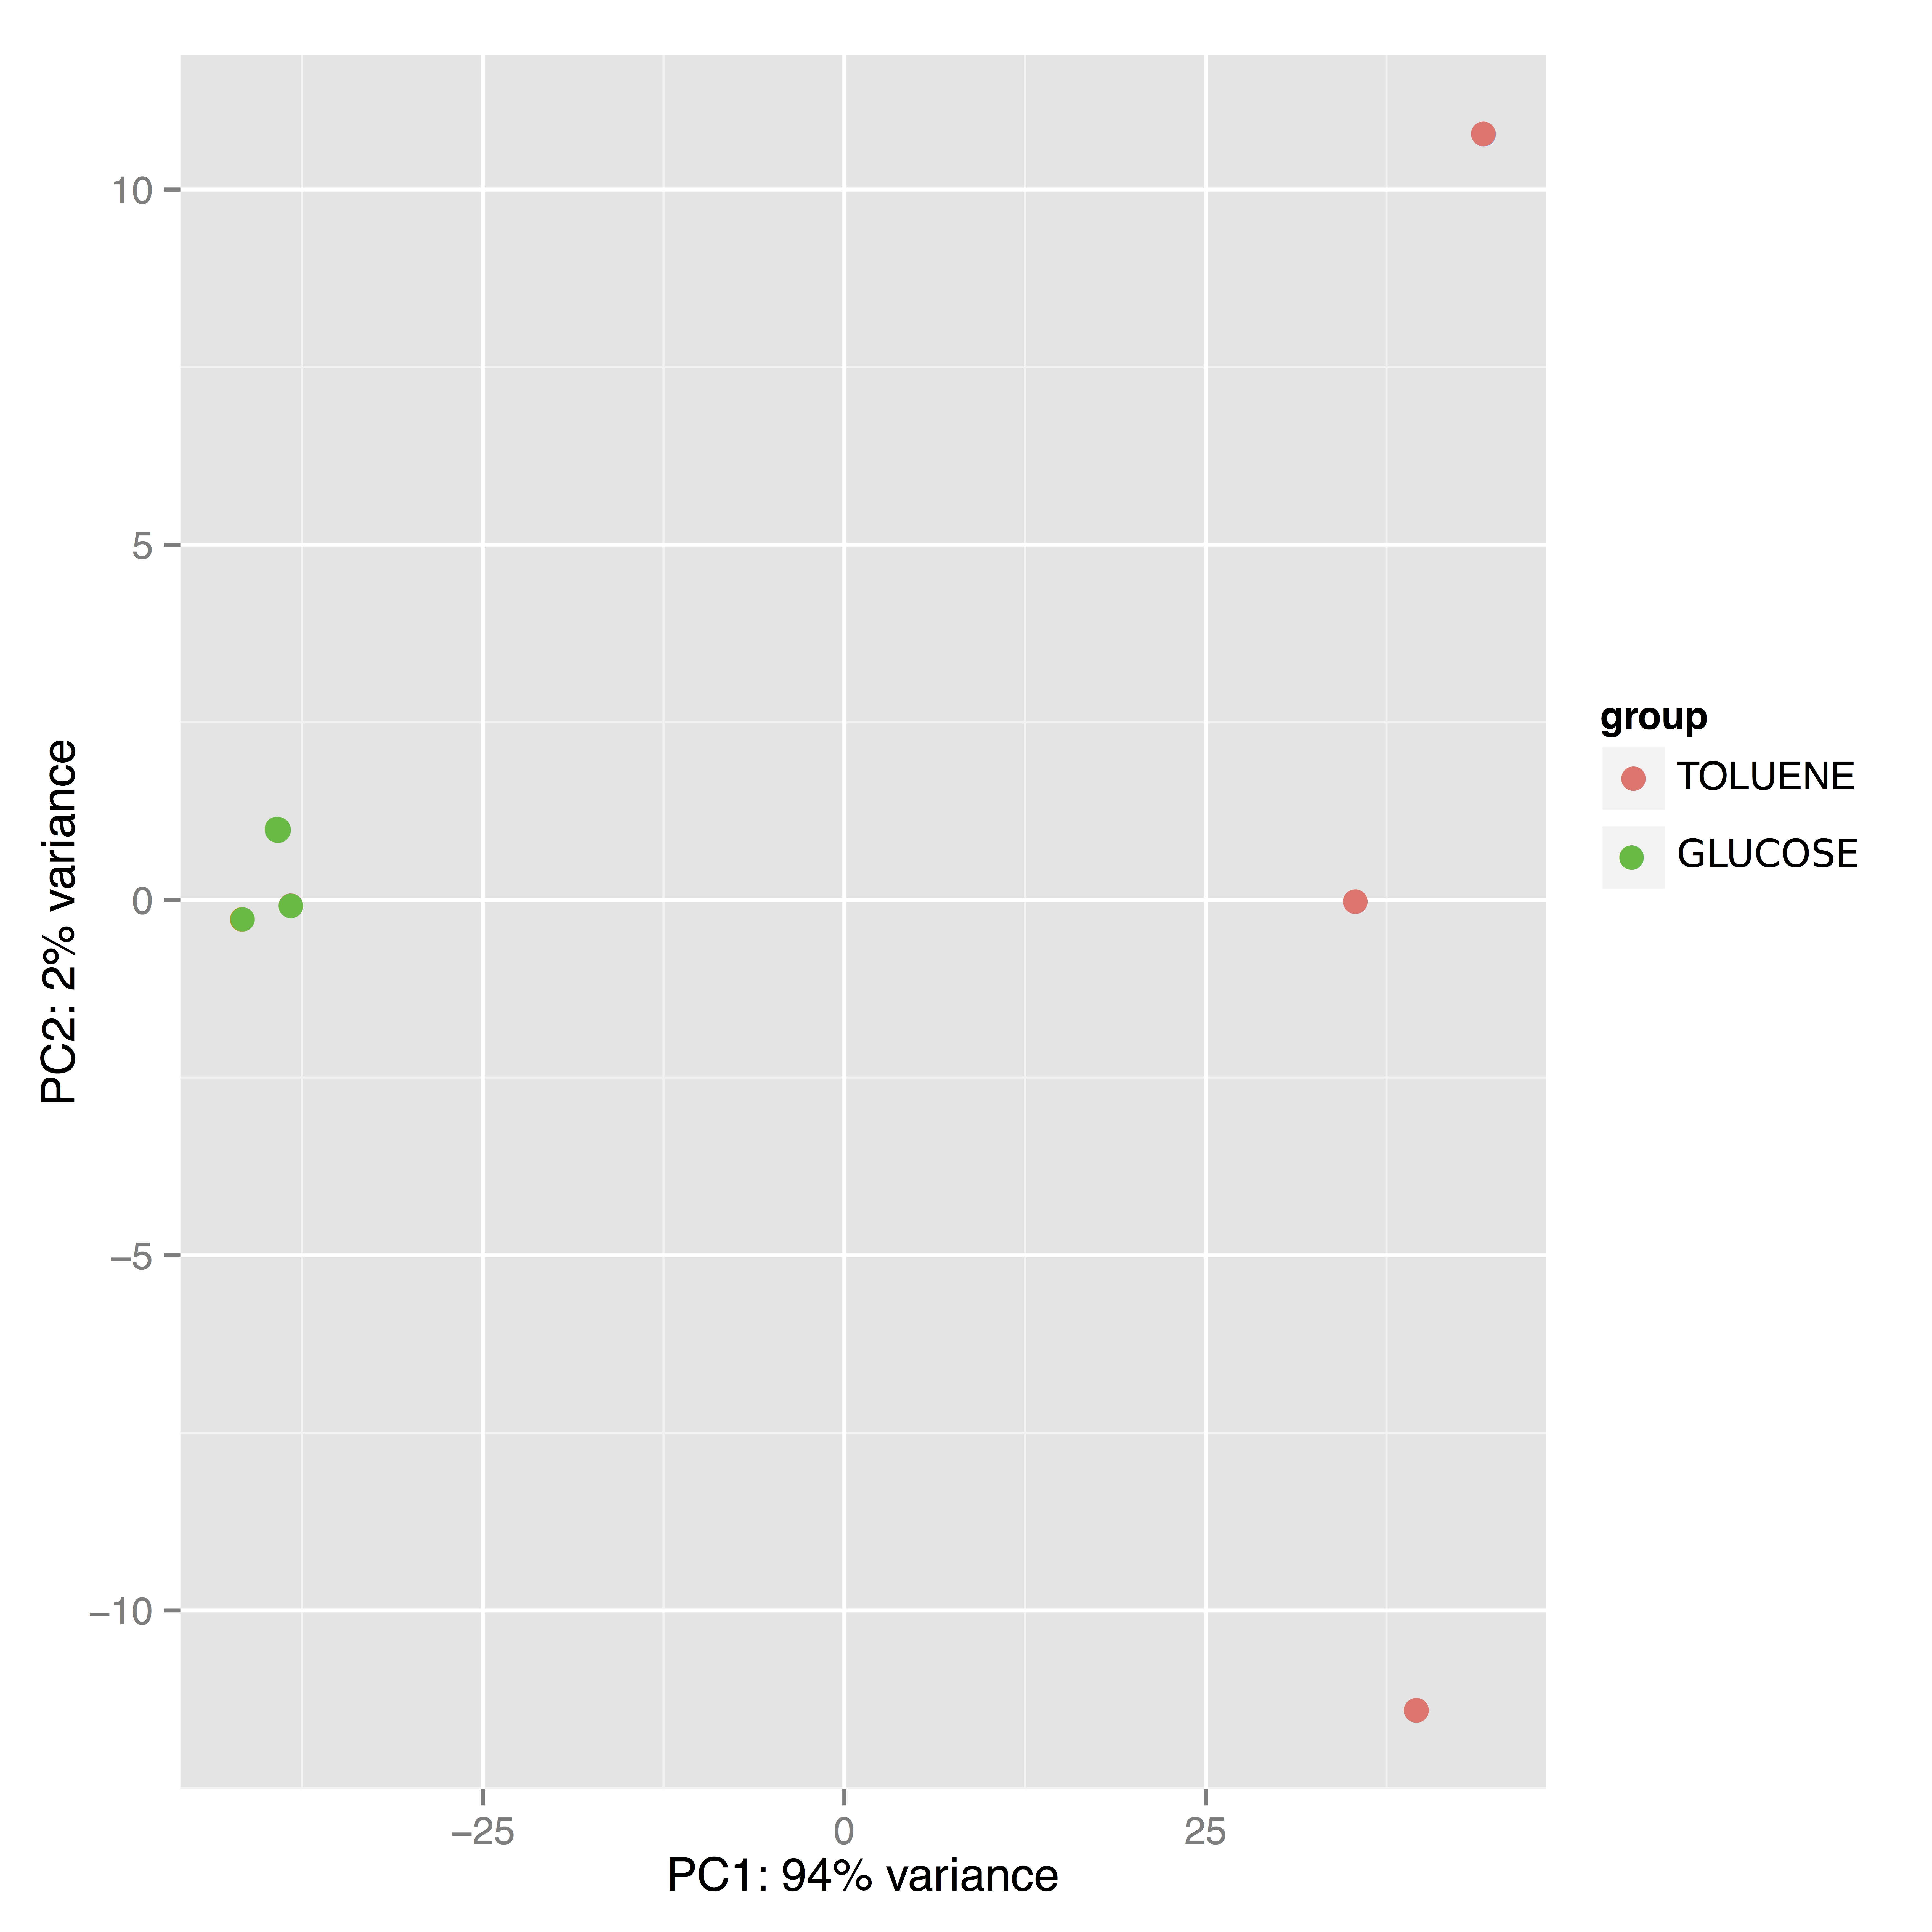
\includegraphics[width=200pt]{pics/PCA2}
		\caption{Principal component analysis} \label{fig:pca}
	\end{subfigure}
	\hspace*{\fill} % separation between the subfigures
	\caption{Correlation analysis} \label{fig:1}
\end{figure}


\newpage
\section{Functional enrichment}

\subsection{Gene Ontology}
Gene Ontology analysis represent the major and minor changes in biological process, cellular component and molecular function. 

\begin{table}[H]
	\centering
	\tiny
\begin{tabular}{c|c|c|c|c|c|p{3,2cm}|c}
	\textbf{ID}&\textbf{P-value}&\textbf{OddsRatio}&\textbf{ExpCount}&\textbf{Count}&\textbf{Size}& \textbf{Term}&\textbf{FDR}\\
	\hline
GO:0019538&	8,97E-06&	2,363104312	&19,74720125&	40&	786&	protein metabolic process	&0,001948953\\
GO:0044267 & 9,21E-06&	2,498080515	&16,20476438&	35&	645	&cellular protein metabolic process&	0,001948953\\
GO:0006457	&4,62E-05	&7,153393393&	1,331554283&	8&	53&	protein folding	&0,00650895\\
GO:0043170	&0,000235609&	1,714121695&	57,0055975&	80&	2269&	macromolecule metabolic process&	0,024915629\\
GO:0044260	&0,000353588&	1,698863684	&53,11142932&	75	&2114&cellular macromolecule metabolic process&	0,029913529\\
GO:0009987	&0,000500955&	1,678863549&	111,5490758&	134	&4440&	cellular process&	0,035317296\\
GO:0006259	&0,000641171& 3,128205128	&4,57250716&	13	&182&	DNA metabolic process&	0,038745034\\
GO:0050896	&0,001207766&	2,309548097	&9,471621973&	20&	377	&response to stimulus&	0,059594894\\
GO:0036211	&0,001408863&	2,39001387	&8,215438688&	18&	327	&protein modification process&	0,059594894\\
GO:0006464	&0,001408863&	2,39001387	&8,215438688&	18&	327	&cellular protein modification process&	0,059594894\\
GO:0051716&	0,001556564&	2,432672441&	7,612470711&	17&	303&	cellular response to stimulus&	0,059856958\\
GO:0043412&	0,001812698&	2,274957274&	9,094766988&	19&	362&	macromolecule modification&	0,060287023\\
GO:0006515&	0,001852793&	78,40837696&	0,075370997&	2&	3&	misfolded or incompletely synthesized protein catabolic process&	0,060287023\\
GO:0006950&	0,002149255&	2,837258893&	4,597630825&	12&	183&	response to stress&	0,0649382\\
GO:0006281&	0,002347231&	3,406839623&	2,889221557&	9&	115&	DNA repair&	0,065846628\\
GO:0006974&	0,002490653&	3,374542869&	2,914345223&	9&	116&	cellular response to DNA damage stimulus&	0,065846628\\
GO:0043038&	0,003061277&	5,664133739&	1,004946628&	5&	40&	amino acid activation&	0,068153683\\
GO:0043039&	0,003061277&	5,664133739&	1,004946628&	5&	40&	tRNA aminoacylation&	0,068153683\\
GO:0006418&	0,003061277&	5,664133739&	1,004946628&	5&	40&	tRNA aminoacylation for protein translation&	0,068153683\\
GO:0033554&	0,00331557&	3,221710016&	3,039963551&	9&	121&	cellular response to stress&	0,068335305\\
GO:0044237&	0,003392533&	1,503857005&	73,28573288&	92&	2917&	cellular metabolic process&	0,068335305\\
GO:0071704&	0,00385927&	1,490845061&	82,33025254&	101&	3277&	organic substance metabolic process&	0,074203235\\
GO:0016569&	0,004632185&	10,73397129&	0,35173132&	3&	14&	covalent chromatin modification&	0,081642257\\
\hline
\end{tabular}
\caption{Overrepresented GO terms for the genes up-regulated}
\label{tab:GOup}
\end{table}

The results, as shown in table \ref{tab:GOup}, indicate that there are changes in the protein metabolic process and cellular protein metabolic process. Because of that, chemical reactions and pathways involving a specific protein, e.g. protein modifications, are higher expressed. 
%\HT{UNKLAR:There is an impact on the chemical reactions and pathways involving a specific protein, rather than of proteins in general.} \\
Protein folding is the next up-regulated process, which affect the chaperone activity. Chaperones assist in the covalent and non-covalent assembly of single chain polypeptides into the correct tertiary structure. \\
Furthermore the metabolic processes of macromolecules, cellular macromolecules, DNA and the protein modification process are up-regulated. The significance of these processes is lower than in the first three processes. In figure \ref{fig:goup} the results obtained from the GO terms for up-regulated genes are presented. 

\begin{figure}[H]
	\centering	
	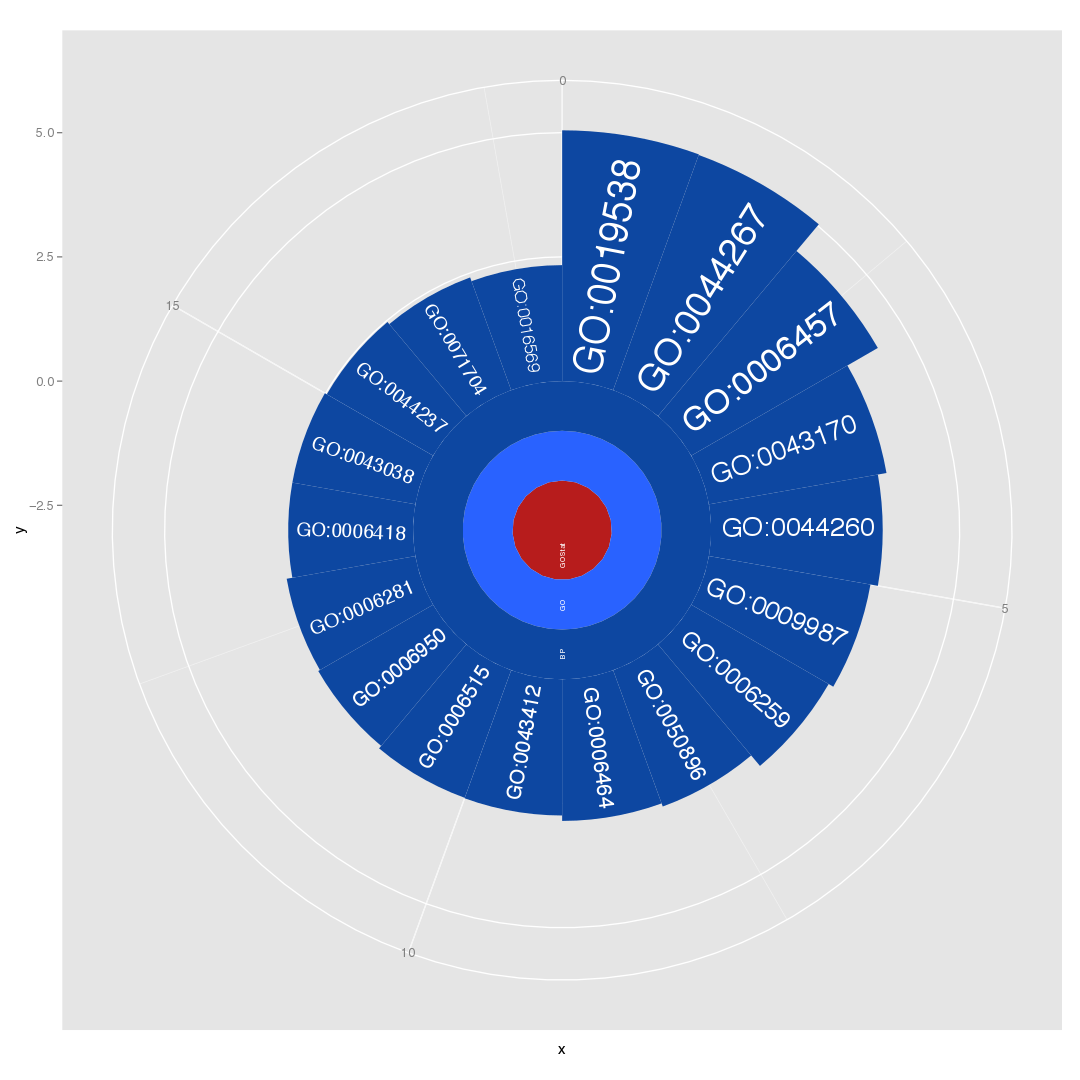
\includegraphics[width=420pt]{pics/GO_Up2.png}
	\caption[GO terms for up-regulated genes]
	{GO terms for up-regulated genes}
	\label{fig:goup}
\end{figure}

\begin{table}[H]
	\centering
	\tiny
	\begin{tabular}{c|c|c|c|c|c|p{4cm}|c}
		\textbf{ID}&\textbf{P-value}&\textbf{OddsRatio}&\textbf{ExpCount}&\textbf{Count}&\textbf{Size}& \textbf{Term}&\textbf{FDR}\\
		\hline
GO:0006412&	1,40E-25&	9,962993421&	6,69317886&	45&	197&	translation&	8,67E-23\\
GO:0006091&	6,42E-20&	28,14456522&	1,494923197&	21&	44&	generation of precursor metabolites and energy&	1,99E-17\\
GO:0046128&	4,66E-15&	21,47353142&	1,392996615&	17&	41&	purine ribonucleoside metabolic process&	7,24E-13\\
GO:0042278&	4,66E-15&	21,47353142&	1,392996615&	17&	41&	purine nucleoside metabolic process&	7,24E-13\\
GO:0009199&	1,15E-14&	28,22027439&	1,053241343&	15&	31&	ribonucleoside triphosphate metabolic process&	1,01E-12\\
GO:0009144&	1,15E-14&	28,22027439&	1,053241343&	15&	31&	purine nucleoside triphosphate metabolic process&	1,01E-12\\
GO:0009205&	1,15E-14&	28,22027439&	1,053241343&	15&	31&	purine ribonucleoside triphosphate metabolic process&	1,01E-12\\
GO:0046034&	1,30E-14&	34,99527665&	0,883363707&	14&	26&	ATP metabolic process&	1,01E-12\\
GO:0044281&	2,50E-14&	3,67855516&	20,96290029&	60&	617&	small molecule metabolic process&	1,73E-12\\
GO:0009141&	3,74E-14&	25,07791328&	1,121192398&	15&	33&	nucleoside triphosphate metabolic process&	2,32E-12\\
GO:0072521&	2,67E-13&	12,3180939&	2,242384796&	19&	66&	purine-containing compound metabolic process&	1,43E-11\\
GO:0009167&	2,99E-13&	20,50720621&	1,257094507&	15&	37&	purine ribonucleoside monophosphate metabolic process&	1,43E-11\\
GO:0009126&	2,99E-13&	20,50720621&	1,257094507&	15&	37&	purine nucleoside monophosphate metabolic process&	1,43E-11\\
GO:0009119&	3,35E-13&	15,13729508&	1,732751888&	17&	51&	ribonucleoside metabolic process&	1,49E-11\\
GO:0015980&	4,19E-13&	29,87096774&	0,883363707&	13&	26&	energy derivation by oxidation of organic compounds&	1,74E-11\\
GO:0045333&	8,81E-13&	35,71566265&	0,747461599&	12&	22&	cellular respiration&	3,42E-11\\
GO:0009150&	1,70E-12&	15,07959184&	1,630825306&	16&	48&	purine ribonucleotide metabolic process&	6,21E-11\\
GO:0019693&	2,45E-12&	14,62065553&	1,664800833&	16&	49&	ribose phosphate metabolic process&	8,00E-11\\
GO:0009259&	2,45E-12&	14,62065553&	1,664800833&	16&	49&	ribonucleotide metabolic process&	8,00E-11\\
GO:0009161&	2,70E-12&	16,69828365&	1,426972143&	15&	42&	ribonucleoside monophosphate metabolic process&	8,39E-11\\
GO:0009123&	5,92E-12&	15,54247267&	1,494923197&	15&	44&	nucleoside monophosphate metabolic process&	1,75E-10\\
GO:0044711&	9,25E-12&	4,11027424&	11,9933611&	40&	353&	single-organism biosynthetic process&	2,59E-10\\
GO:0006163&	9,60E-12&	13,032984&	1,800702942&	16&	53&	purine nucleotide metabolic process&	2,59E-10\\
GO:0009116&	1,86E-11&	9,169749442&	2,785993231&	19&	82&	nucleoside metabolic process&	4,82E-10\\
GO:1901657&	2,35E-11&	9,025245351&	2,819968758&	19&	83&	glycosyl compound metabolic process&	5,83E-10\\
GO:0006818&	2,93E-11&	18,47158218&	1,155167925&	13&	34&	hydrogen transport&	6,75E-10\\
GO:0015992&	2,93E-11&	18,47158218&	1,155167925&	13&	34&	proton transport&	6,75E-10\\
GO:0042451&	5,71E-11&	20,98936924&	0,985290289&	12&	29&	purine nucleoside biosynthetic process&	1,22E-09\\
GO:0046129&	5,71E-11&	20,98936924&	0,985290289&	12&	29&	purine ribonucleoside biosynthetic process&	1,22E-09\\
GO:1902600&	9,24E-11&	19,8206158&	1,019265816&	12&	30&	hydrogen ion transmembrane transport&	1,91E-09\\
GO:0098660&	2,05E-10&	9,163129391&	2,480213486&	17&	73&	inorganic ion transmembrane transport&	3,85E-09\\
GO:0098662&	2,05E-10&	9,163129391&	2,480213486&	17&	73&	inorganic cation transmembrane transport&	3,85E-09\\
GO:0098655&	2,05E-10&	9,163129391&	2,480213486&	17&	73&	cation transmembrane transport&	3,85E-09\\
GO:0044267&	2,39E-10&	3,014787023&	21,91421505&	54&	645&	cellular protein metabolic process&	4,36E-09\\
GO:0009117&	3,44E-10&	6,995755234&	3,635381411&	20&	107&	nucleotide metabolic process&	6,11E-09\\
GO:0015672&	3,82E-10&	10,71283391&	1,936605051&	15&	57&	monovalent inorganic cation transport&	6,59E-09\\
GO:0009142&	4,38E-10&	26,83810214&	0,713486071&	10&	21&	nucleoside triphosphate biosynthetic process&	6,64E-09\\
GO:0009145&	4,38E-10&	26,83810214&	0,713486071&	10&	21&	purine nucleoside triphosphate biosynthetic process&	6,64E-09\\
GO:0009201&	4,38E-10&	26,83810214&	0,713486071&	10&	21&	ribonucleoside triphosphate biosynthetic process&	6,64E-09\\
\hline
	\end{tabular}
	\caption{Overrepresented GO terms for the genes down-regulated}
	\label{tab:GOdown}
\end{table}

The biological process of translation is down-regulated. Translation is the synthesis of proteins and therefore one of the most important process within a cell.\\
The chemical reactions and pathways resulting in the formation of precursor metabolites and substances, from which energy is derived, are also down-regulated. \\

As can be seen in table \ref{tab:GOdown}, most overrepresented GO terms belong to the purine nucleoside metabolic process. A nucleoside or ribonucleoside bound to a triphosphate are also know as GTP (guanosine triphosphate) or ATP (adenosine triphosphate) and are necessary for cell metabolism and regulation, especially those involving DNA and RNA synthesis. They act as energy source or activator for substrates.\\
Additionally, genes for the ATP metabolic process and the proton transport are lower expressed significantly. The mentioned processes belong to generation of energy. 
\begin{figure}[H]
	\centering	
	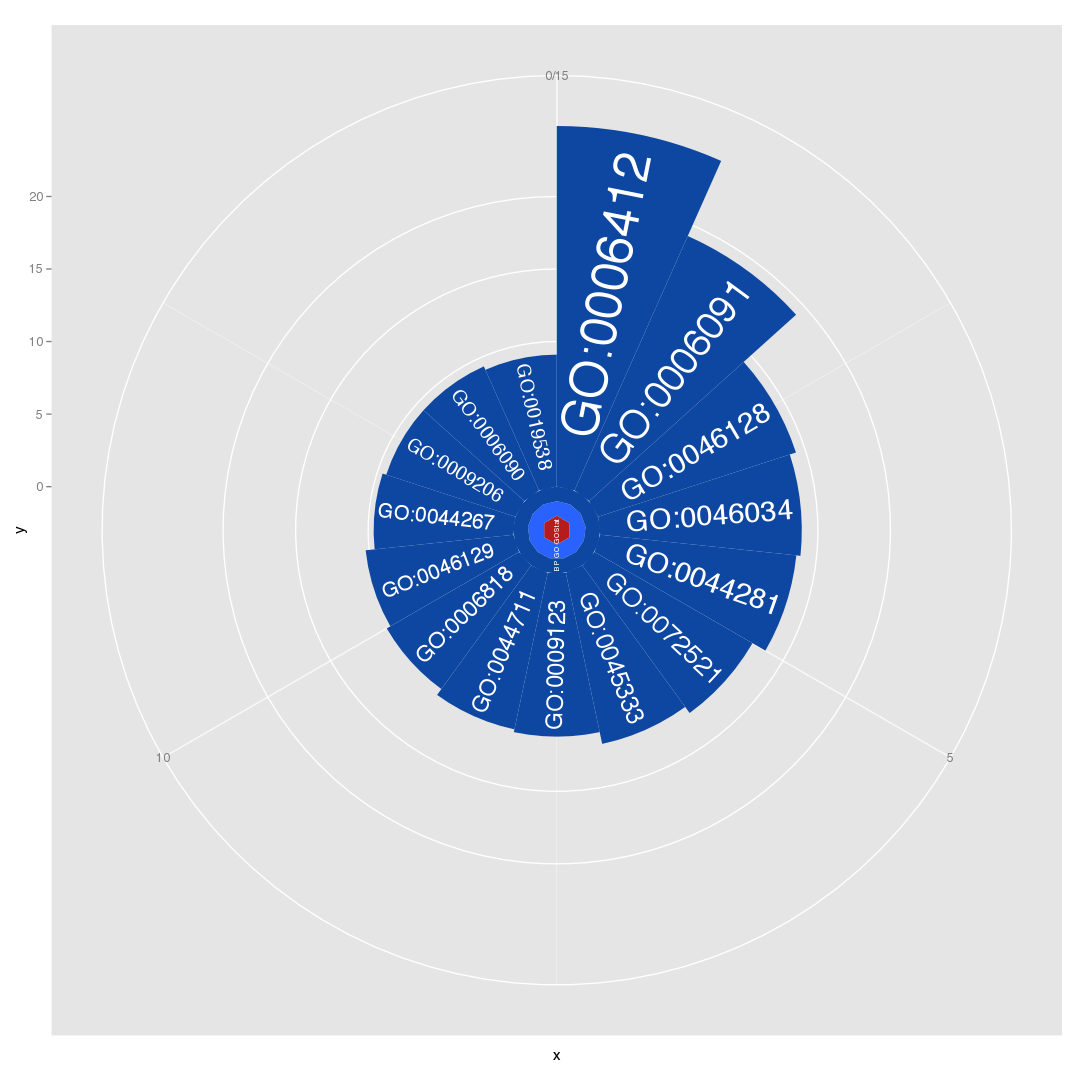
\includegraphics[width=300pt]{pics/GO_Down2.png}
	\caption[GO terms for down-regulated genes]
	{GO terms for down-regulated genes}
	\label{fig:godown}
\end{figure}

In figure \ref{fig:godown} the results obtained from the GO terms for lower expressed genes are presented. Similar processes, like purine ribonucleoside metabolic process and purine nucleoside metabolic process, are grouped together. 


\subsection{KEGG}

\begin{table}[H]
	\centering
	\tiny
	\begin{tabular}{c|c|c|c|c|c|c|p{2cm}}
		\textbf{ID}&\textbf{P-value}&\textbf{OddsRatio}&\textbf{ExpCount}&\textbf{Count}&\textbf{Size}& \textbf{FDR}&\textbf{Fenes}\\
		\hline
ko00020&	0,000297044&	30,4&	0,436363636	&4	&6&	0,008614271	&JSEJ01000010.1.81 JSEJ01000023.1.136 JSEJ01000099.1.18 JSEJ01000099.1.19\\
\hline
ko00660&	0,00065906&	20,2&	0,509090909&	4&	7&	0,009556376	&JSEJ01000010.1.81 JSEJ01000023.1.136 JSEJ01000099.1.18 JSEJ01000099.1.19\\
\hline
ko00010&	0,001298374&	43,57142857&	0,290909091&	3&	4&	0,012550945&JSEJ01000039.1.14 JSEJ01000027.1.103 JSEJ01000074.1.37\\
		\hline
	\end{tabular}
	\caption{Overrepresented KEGG pathways for the genes down-regulated}
\end{table}
\ \\
%%%% general overview about up and down regulated genes
In contrast to the GO analysis, enrichment of KEGG terms was only found for the down-regulated genes. \\
Genes related to pathways of TCA cycle, carbohydrate metabolism and Glycolysis/Gluconeogenis were lower expressed. These pathways are assigned to carbohydrate and energy categories that function in catabolism.\\
Four genes are differentially expressed in TCA cycle and in C5-branched dibasic acid metabolism. TCA cycle is a central metabolic pathway that completes the oxidative degradation of carbohydrates, amino acids and fatty acids. The energy generated in this cycle is in the form of GTP and ATP. \\
Glycolysis/gluconeogenesis provide the catabolized nutrients as substrates for TCA cycle and C5-branched dibasic acid metabolism. In glycolysis glucose is broken down in pyruvate by production of ATP. Gluconeogenesis is the biosynthesis of glucose from pyruvate and therefore the reverse anabolic process and equal important as glycolysis. \\
Taken together, these results of down-regulated pathways suggets a general shutdown of carbohydrate catabolism and energy generation.

%\begin{figure}[H]
%	\centering	
%	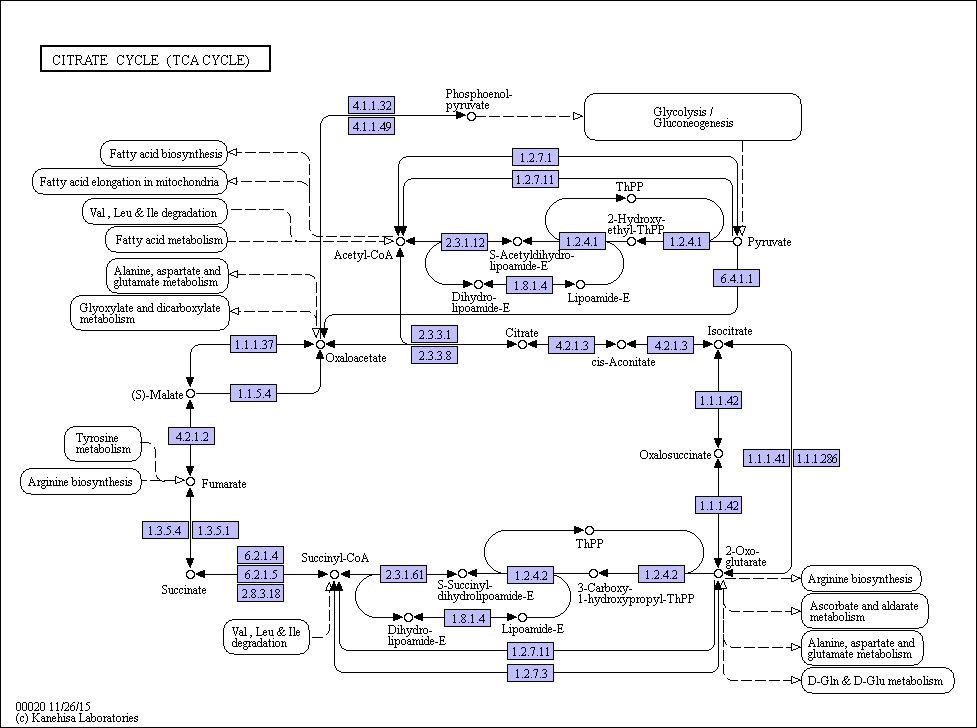
\includegraphics[width=320pt]{pics/tcacycle}
%	\caption[KEGG pathway of TCA cycle]
%	{KEGG pathway of TCA cycle}
%	\label{fig:tcacycle}
%\end{figure}

\subsection{Protein domain enrichment}
Results of differentially expressed proteins were generated with different databases and sequence analysing tools (Pfam, Interpro, UniPath, superfam,...).\\
\ \\
Genes coding for the specific protein Hsp 20 which belong to the family of heat shock proteins are significantly higher expressed in toluene. The synthesis of this proteins is the response to environmental stress. Heat shock proteins act as protein chaperones that can protect protein against denaturation and aggregation \cite{Lindquist1988, Maaroufi2013}. \\
Further, the analysis confirm the up-regulation of proteins coding for HSP20-like chaperones, HSP40/DnaJ peptide-binding and Hsp20 domain. Zinc finger domains (RING/FYVE/PHD-type, CCCH-type) are strongly represented. Zinc finger domains are known as a DNA-binding motif and are involved in transcriptional processes.\\
Interestingly protein coding for AAA+ ATPase domain and ATPase  AAA-type core also are up-regulated. AAA+ ATPase domain participate in diverse cellular processes including membrane fusion, proteolysis and DNA replication. ATPase  AAA-type core function as molecular chaperones and act as DNA helicases and transcription factor.\\
\ \\
In line with the results of KEGG pathway analysis, the enzymes citrate synthase, ATP synthase and CoA-ligase are down-regulated. \\
Citrate synthase catalysis the first reaction in the TCA cycle, the conversion of oxalacetate and acetyl-coenzyme A into citrate and coenzyme A. This reaction is important for energy generation and for carbon assimilation. ATP synthases are a membrane-bound enzyme complexes and ion transporters that combine ATP synthesis and hydrolysis with the transport of protons across the membrane. CoA-ligase is part of succinyl-CoA synthetase and this enzyme belong to TCA cycle. \\
Another lower expressed enzyme is chitin synthase. Chitin synthase catalyzes the conversion of UDP-N-acetyl-D-glucosamine to UDP. UDP is an important factor in gluconeogenesis. \\


\newpage
\section{Toluene Degradation}
%Toluen Pathway 
The result of the previous studies, explained in \ref{study}, indicate that the increase of CO$_2$ concentration come along with the degradation of toluene and \textit{C. immunda} can use toluene as carbon and energy source. Therefore the focus of the results is on the enzymes of the toluene-degradation pathway.\\
The pathway (figure \ref{ToluendegUPDOWN}) starts with an oxidation on the methyl group of toluene, which is catalyzed by cytochrome P-450 monooxygenase (P450) to form benzyl alcohol, which is then converted to benzaldehyde and benzoate by the relevant dehydrogenases (BADH and BZDH). Benzoate is then hydroxylated (BH) to form p-hydroxybenzoate, which is oxidized by p-hydroxybenzoate hydroxylase (PHBH) to protocatechuate. At this stage there are two options, both of which may be occuring simultaneously. Since the organism has P340 activity (protocatechuate-dioxygenase), protocatechuate is likely being metabolized through an ortho-cleavage pathway, which has been seen previously in other fungi. However, since C12O (catechol-1-2-dioxygenase) activity is also present in toluene-grown cells, protocatechuate may be decarboxylated to catechol, which is then oxidized through the other branch of the b-ketoadipate pathway.  The conversion of b-carboxymuconate to b-ketoadipate involves the participation of two enzymes (CMLE and CMH) \cite{Parales2008}. \\

 %%%%%picture of toluene degradation with up/down
 \begin{figure}[H]
 	\centering	
 	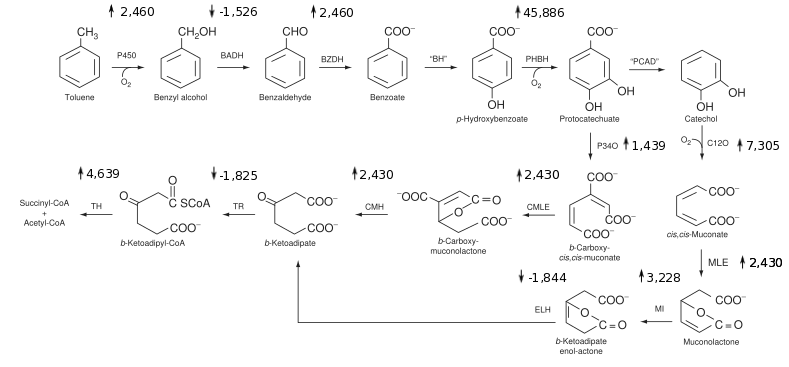
\includegraphics[width=400pt]{pics/toldeg_UPDOWN.png}
 	\caption[Toluene degradation pathway]
 	{Toluene degradation pathway. The values above the enzymes indicate the foldChange.}
 	\label{ToluendegUPDOWN}
 \end{figure}

All but three enzymes (BADH, EHL and TR) of toluene-degradation pathway are up-regulated (figure \ref{ToluendegUPDOWN}). The enzyme with the highest activity is p- hydroxybenzoate hydroxylase. The foldChange-value of enzyme C120 is higher too. In the study of Parales about diversity of microbial toluene degradation \cite{Parales2008} is mentioned that there three genes of the pathway are missing in \textit{C. immunda}. The results of transcriptome analysis indicate a signal for this missing genes, named p-hydroxybenzoate-hydroxylase (PHBH), mucolactone-isomerase (MI), $\beta$- ketoadipateenol -lactonehydrogenase (ELH). Especially the foldChange of PHBH is elevated.
\\
The end products of toluene degradation (Succinyl-CoA and Acetyl-CoA) are utilized as substrates for the TCA cycle. \\
Table \ref{tolenzymes} shows the summary statistic for the enzymes of toluene degradation. \\

%%%%enzymes fo toldegradation
\begin{table}[ht]
	\centering 
	\tiny
	\begin{tabular}{c p{4cm}|c|c|c}
		& \textbf{Enzymes}& \textbf{logFC} & \textbf{P.Value} & \textbf{adj.P.Value} \\
		\hline
		\textbf{P450} & Cytochrome-P-450 toluene monooxygenase & 1.2991421176278 & 4.76275764901422x10$^5$ & 0.00015206178906281 \\
		\hline
		\textbf{BADH} & Benzyl-Alcohol-Dehydrogenase & -0.610068198027962 & 0.0215490685115476 & 0.0341873128136395 \\
		\hline
		\textbf{BZDH} & Benzal-Dehydrogenase & 1.29914211762787 & 4.76275764901422x10$^5$ & 0.000152061789062813 \\
		\hline
		\textbf{BH} & hypothetical-Benzoate-Hydroxylase & & & \\
		\hline
		\textbf{PHBH} & p-hydroxybenzoate-Hydroxylase & 5.52538725225511 & 1.45988708444616x10$^-10$ & 7.61270285910155x10$^-9$  \\
		\hline
		\textbf{PCAD} & Protocatechuate-Dioxygenase & & & \\
		\hline
		\textbf{C120} & Catechol-1-2-Dioxygenase & 2.86929824283322 & 2.88989072866634x10$^-6$ & 1.43614755006986x10$^-5$ \\
		\hline
		\textbf{MLE} & cis-cis-Muconate-Lactonizing-Enzyme & 1.28113181586883 & 0.00654904836295034 & 0.0117901712197061 \\
		\hline
		\textbf{MI} & Mucolactone-Isomerase & 1.6912116141732 & 0.00111759914912401 & 0.0024233473897696 \\
		\hline
		\textbf{ELH} & $\beta$-ketoAdipateEnol-LactoneHydrogenase & -0.883899764697411 & 0.0121983401347394 & 0.0205651854673907 \\
		\hline
		\textbf{P340} & Protocatechuate-Dioxygenase & & & \\
		\hline
		\textbf{CMLE} & $\beta$-Carboxy-cis-cis-Muconate-Lactonizing-Enzyme & 1.28113181586883 & 0.00654904836295034 & 0.0117901712197061 \\
		\hline
		\textbf{CMH} & $\beta$-Carboxymuconate-Enzyme &  1.28113181586883 & 0.00654904836295034 & 0.011790171219706 \\
		\hline
		\textbf{TR} & $\beta$-ketoadipat-CoA-Transferase & -0.868139308745568 & 0.0167231462329001 & 0.0272631578512478 \\
		\hline
		\textbf{TH} & $\beta$-ketoadipyl-CoA-Thiolase & 2.2148894022903 & 2.73997262728265x10$^-7$ & 2.13649579005871x10$^-6$ \\ 
		\hline	
	\end{tabular}
	\caption{Enzymes of toluene degradation}
	\label{tolenzymes}
\end{table}


%\subsection{Melanin synthesis}
%Melanin is a pigment found in all biological kingdoms. Knowing that melanin defends against environmental stresses such as ultraviolet light, oxidizing agents and ionizing radiation, it contributes to the ability of fungi to survive in harsh environments.  The second important thing about melanin production by fungi is the virulence of pathogens of humans. \cite{Golde1991} 
% \begin{figure}[H]
% 	\centering	
% 	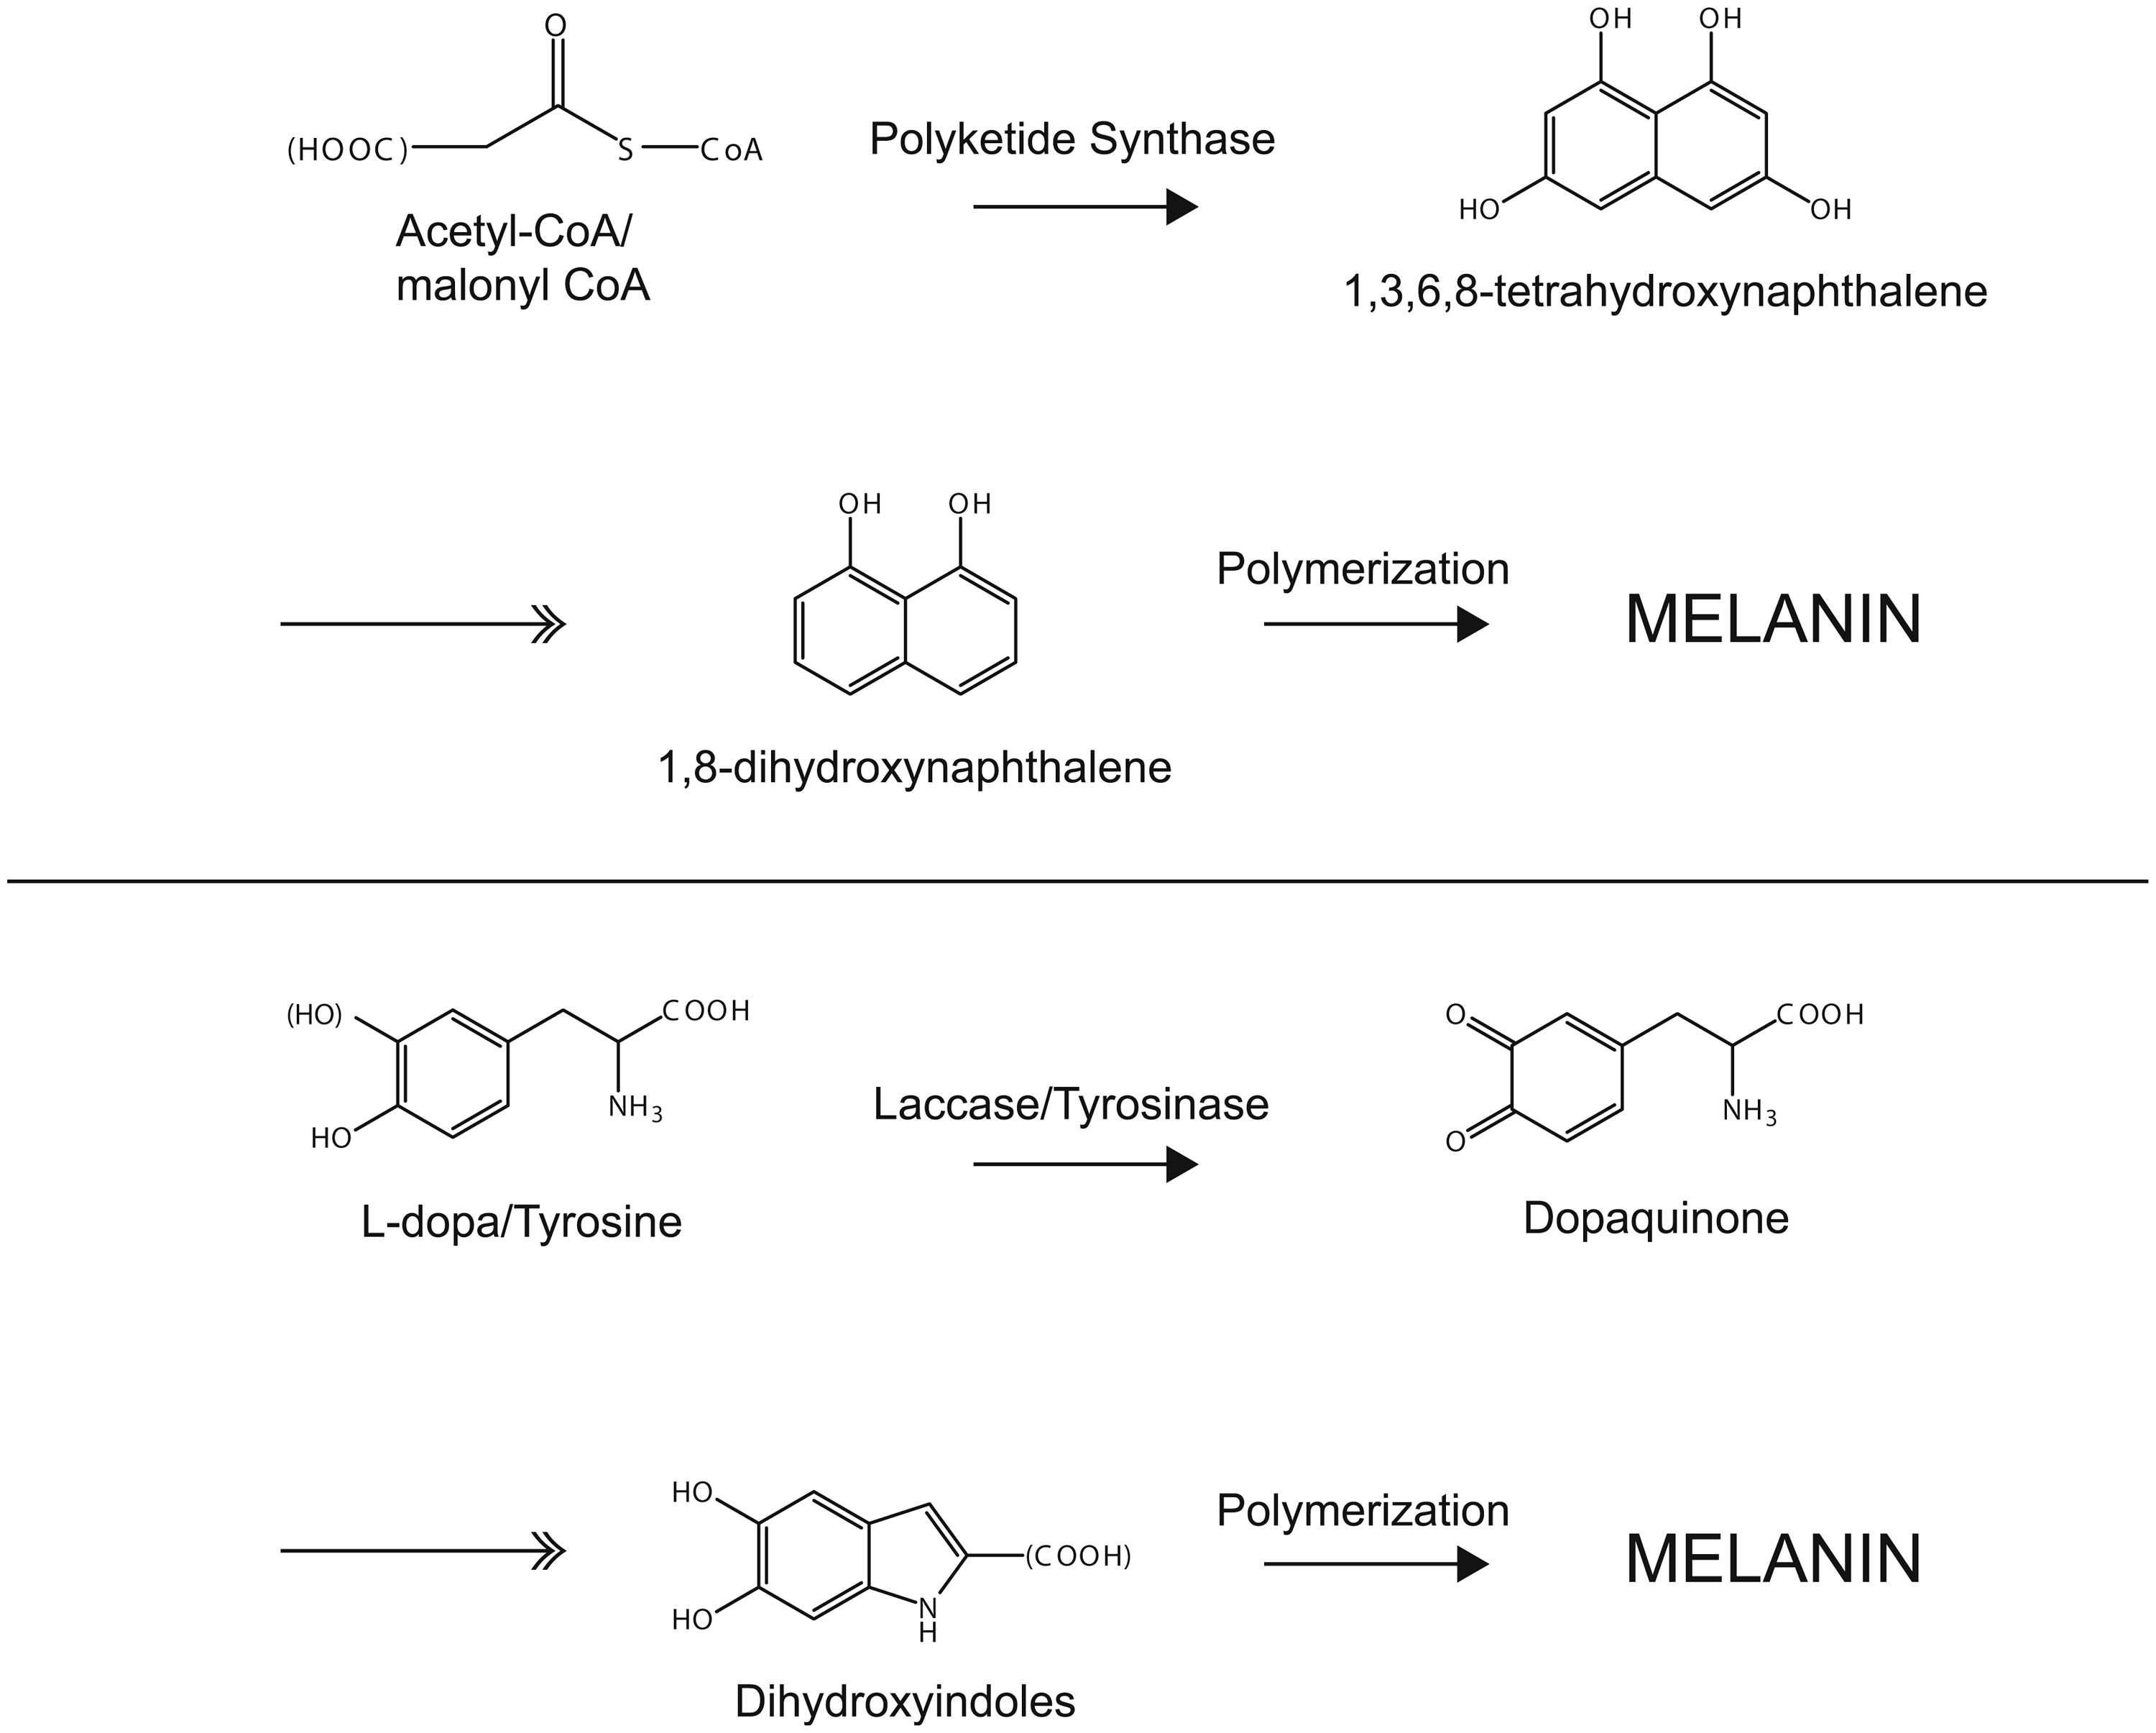
\includegraphics[width=350pt]{pics/melaninsynthesis.png}
% 	\caption[Melanin synthesis pathway in fungi]
% 	{Melanin synthesis pathway in fungi}
% 	\label{melanin}
% \end{figure}
%In the melanin synthesis pathway the first step is the formation of 1,3,6,8- tetrahydroxynaphthalene (1,3,6,8-THN) catalysed by a polyketide synthase (PKS). Followed by series of of reduction and dehydration reactions the intermediates scytalone, 1,3,8- trihydroxynaphthalene, vermelone, and finally 1,8- dihydroxynaphthalene (DHN) are produced. Finally polymerization of DHN leads to formation of melanin. \cite{Golde1991}
%
%\begin{table}[H]
%	\centering
%	\begin{tabular}{|c p{6cm}|c|c|c|}
%		\hline
%		& \textbf{Enzymes} & \textbf{logFC} & \textbf{P.Value} & \textbf{adj.P.Value} \\
%		\hline
%		\textbf{PKS} & Polyketide Synthase & & & \\
%		\hline
%	\end{tabular}
%	\caption{Enzymes of melanin synthesis}
%\end{table}



\newpage
\setcounter{chapter}{4}\setcounter{section}{0}
\chapter*{Discussion}
\addcontentsline{toc}{chapter}{Discussion}
The study was designed to determine the effect of toluene on \textit{C. immunda} at transcriptome level and use its degrading performances in biotechnological applications like bioremediation \cite{BarbaraBlasi2015}. Previous results indicated that \textit{C. immunda} has the ability to degrade toluene and use it as sole carbon source, confirmed through an increase in CO$_2$-concentration \cite{Poyntner2014}. The present work provides information on gene expression changes observed during the response to using toluene as sole carbon source.\\
Overall, the study found out that regulation of transcription and translation are significantly down-regulated. This result may be explained by the fact that the addition of toluene to the media causes a stress situation for the cell. Biological processes and pathways relating to cell metabolism and energy generation are expressed less frequently compared to glucose-samples, e.g. carbohydrate metabolism and TCA cycle. TCA cycle is the central metabolic pathway for ATP production within a cell and provides the precursors for biosynthesis of various metabolic products. Processes relating to the purine nucleoside metabolic process have a lower expression, which in addition has an effect on the cell metabolism and energy generation too. Together these results shows that the fungi is probably saving energy during stress situations. This observation is corroborated by the down-regulation of carbon metabolism and supports the idea that \textit{C. immunda} use toluene as an energy source. \\
According to these data, genes coding for DNA-binding motifs like Zinc finger are up-regulated. Zinc finger proteins are transcription factors capable of binding selectively to specific sequences of DNA. They can act as repressor or activator of the transcription. Further studies of \textit{C. immunda} could be used to determine if Zinc finger proteins support or prevent transcription. \\
The positive response to the stress is related to up-regulated genes. These include genes predicted to be involved in chaperone protein folding activity and DNA repair and thus, protection of the cell. The genes coding for specific protein metabolic processes and protein folding are highly expressed. Toluene is a stress factor leading to protein folding machinery. This may reflect the tolerance of this fungi exhibit by building heat shock proteins. \\
The predicted genes that are essential for the category of glycolysis/gluconeogenesis are down-regulated. 
Gluconeogenises is needed when glucose is not longer available, this suggests that \textit{C. immunda} use an alternate carbon source metabolism. It can therefore be assumed that the missing catabolites from glycolysis and gluconeogenises are provided by the products of toluene degradation.\\

These categories of differentially expressed genes show an opposing regulation pattern after toluene-treatment. The results of GO enrichment and KEGG pathways analysis revealed a coordinated shutdown of metabolic activity at the transcriptome level. The cell slows down the processes of RNA synthesis and subsequent protein synthesis, but can survive by building proteins for protection. 
So the stress response and defense strategies are adapting during this condition. This might even mean that toluene concentrations were way too high leading to the dormant state. In contrast \textit{Cladophialophora immunda} has the ability to degrade toluene. \\
Genes coding for enzymes necessary for toluene degradation are generally up-regulated. Fungi with the ability to grow on aromatic hydrocarbons might contribute to bioremediation of BTEX mixture. Therefore this fungi is a candidate for bioremediation through the ability to use toluene as sole carbon source and degrade it. This would be a fruitful area for further research of fungal bioremediation. \\

The implementation of workflow system for genome annotation with RNA-seq data was sucessful. It is a fast method to analyse transcriptomics data that allow annotations of coding and non-coding genes and gene expression analysis. The pipeline can be used for analysing other transcriptomics data of black yeasts.\\

\newpage
\chapter*{Conclusion}
\addcontentsline{toc}{chapter}{Conclusion}
The aim of this work was to study the transcriptional response of \textit{Cladophialophora immunda} when exposed to toluene as the sole carbon source. This extremophilic organism is an important fungi with the ability to degrade toluene. \textit{Cladophialophora immunda} can use toluene as a carbon and energy source  and provide these catabolites as substrates for the TCA cycle. \\

For analysis, a genome annotation pipeline with RNA-seq data as input was developed. This pipeline allows the fast and reproductible study of transcriptomics data, like differential expression, coding and non-coding gene annotation. It should be noted that the softwares and differential expression analysis methods used for RNA-seq are still under active development. RNA-seq has clear advantages over other methods like microarrays. The future challenge is to target more complex transcriptomes and without the matching software, analysing transcriptome is not possible. \\
 
Possibilities for ongoing research could to look more closely at enzymes of toluene degradation pathway or special proteins by PCR methods to get a deeper understanding of the black yeasts such as special \textit{Cladophialophora immunda}.\\
 

\newpage
The equipment of the VIBT-Extremophile Center used in this study was financed by BOKU-Equipment GesmbH. The computational results presented have been achieved in part using the Vienna Scientific Cluster (VSC). \\
\newpage
%\bibliography{/Users/christina/Documents/Bibtex/Masterthesis}
%\bibliographystyle{plain}
\bibliography{bib/library}
\addcontentsline{toc}{chapter}{Bibliography}
\newpage
\listoffigures
\addcontentsline{toc}{chapter}{List of Figures}
\newpage
\listoftables
\addcontentsline{toc}{chapter}{List of Tables}
\newpage
\vspace{2cm}

STATUTORY DECLARATION\\
I declare that I have authored this thesis independently, that I have not used
other than the declared sources / resources, and that I have explicitly marked
all material which has been quoted either literally or by content from the used
sources.\\
\vspace{1cm}

EIDESSTATTLICHE ERKLÄRUNG\\
Ich erkläre an Eides statt, dass ich die vorliegende Arbeit selbstständig verfasst,
andere als die angegebenen Quellen/Hilfsmittel nicht benutzt, und die
den benutzten Quellen wörtlich und inhaltlich entnommene Stellen als solche
kenntlich gemacht habe.\\
\vspace{3cm}


Wien, Juni 2016  \hspace*{6cm} Christina Kustor



\end{document}
